\documentclass[12pt, oneside]{book}

%% Language and font encodings
\usepackage[english]{babel}
\usepackage[utf8x]{inputenc}
\usepackage[T1]{fontenc}
\usepackage{amsfonts}

%% Sets page size and margins
\usepackage[a4paper,top=3cm,bottom=2cm,left=3cm,right=3cm,marginparwidth=1.75cm]{geometry}

%% Useful packages
\usepackage{amsmath}
\usepackage{amssymb}
\usepackage{stmaryrd}
\usepackage{amsthm}
\usepackage{graphicx}
\usepackage[colorinlistoftodos]{todonotes}
\usepackage[colorlinks=true, allcolors=blue]{hyperref}
\usepackage{enumitem}
\usepackage{multicol}
\usepackage{tikz, pgfplots}
\usetikzlibrary{positioning}

%Commands definitions
\newcommand{\setbackgroundcolour}{\pagecolor[rgb]{0.1,0.1,0.1}}  
\newcommand{\settextcolour}{\color[rgb]{1,1,1}}    
\newcommand{\invertbackgroundtext}{\setbackgroundcolour\settextcolour}
\newcommand{\dvd}{\mathrel{|}}
\newcommand{\Iint}[2]{\llbracket #1 , #2 \rrbracket}
\newcommand{\Z}[1]{\mathbb{Z} / #1 \mathbb{Z}}
\renewcommand{\phi}{\varphi}
\newcommand{\etoile}[1]{\mathbb{#1}^{\times}}

%Command execution. 
%If this line is commented, then the appearance remains as usual.
%\invertbackgroundtext

% New mathematical operator
\DeclareMathOperator{\Ima}{im}
\DeclareMathOperator{\Ker}{Ker}
\DeclareMathOperator{\lcm}{lcm}
\DeclareMathOperator{\sgn}{sgn}

%Set QED symbol to blacksquare
\renewcommand\qedsymbol{$\blacksquare$}

%% Table packages
\usepackage{array}
\newcolumntype{P}[1]{>{\centering\arraybackslash}p{#1}}
\usepackage{multirow}

% Définir un nouveau compteur d'exercice
\newcounter{exercise}[section] % Compteur qui est remis à zéro à chaque nouvelle section

% Définir un environnement pour l'exercice
\newenvironment{exercise}{
    \refstepcounter{exercise} % Incrémenter le compteur
    \noindent\textbf{Exercise \arabic{exercise}} 
    \\ 
}{} % Fin de l'environnement

% Définir un environnement pour les solutions
\newenvironment{solution}{
    \noindent\textbf{Solution} 
}{}


\title{Solutions to Abstract Algebra (Third Edition)
\\ - David S. Dummit \& Richard M. Foote}
\author{Samy Lahlou}

\begin{document}
\maketitle

\chapter*{Preface}

The goal of this document is to share my personal solutions to the exercises
in the third edition of Abstract Algebra by David S. Dummit and Richard M. Foote
during my reading. \\
As a disclaimer, the solutions are not unique and there will 
probably be better or more optimized solutions than mine. Feel free to 
correct me or ask me anything about the content of this document at the 
following address : samy.lahloukamal@mcgill.ca\\

\tableofcontents

\chapter*{Preliminaries}
\addcontentsline{toc}{chapter}{Preliminaries}
\section{Basics}
\section{Properties of the Integers}
\section{The Integers Modulo $n$}

\part{GROUP THEORY}


% CHAPTER 1
\chapter{Introduction to Groups}
\section{Basic Axioms and Examples}

% CHAPTER 2
\chapter{Subgroups}
\section{Definition and Examples}
\section{Centralizers and Normalizers, Stabilizers and Kernels}

[Pas encore numérisé.]
\section{Cyclic Groups and Cyclic Subgroups}

\begin{exercise}
    Find all subgroups of $Z_{45}=\langle x\rangle$, giving a generator for
    each. Describe the containments between these subgroups.\\
\end{exercise}

\begin{solution}
    \\ First, recall that the positive divisors of $45$ are the following:
    $$1, 3, 5, 9, 15, 45$$
    By Theorem $7$, the subgroups of $Z_{45}$ are exactly $\langle x^d\rangle$
    where $d$ is a divisor. Hence, the subgroups are :
    \begin{itemize}
        \item $\langle x^1\rangle = Z_{45}$
        \item $\langle x^3\rangle = \{1, x^3, x^6, x^9, x^{12}, x^{15},
        x^{18}, x^{21}, x^{24}, x^{27}, x^{30}, x^{33}, x^{36}, x^{39},
        x^{42}\}$
        \item $\langle x^5\rangle = \{1, x^5, x^{10}, x^{15}, x^{20},
        x^{25}, x^{30}, x^{35}, x^{40}\}$
        \item $\langle x^9\rangle = \{1, x^9, x^{18}, x^{27}, x^{36}\}$
        \item $\langle x^{15}\rangle = \{1, x^{15}, x^{30}\}$
        \item $\langle x^{45}\rangle = \{1\}$
    \end{itemize}
    We can represent the inclusions between the subgroups with the following
    diagram:
    \begin{center}
        \begin{tikzpicture}
            %Nodes
            \node at (4,0) (1) {$Z_{45}$};
            \node at (2,-2) (3) {$\langle x^3\rangle$};
            \node at (6,-2) (5) {$\langle x^5\rangle$};
            \node at (0,-4) (9) {$\langle x^9\rangle$};
            \node at (4,-4) (15) {$\langle x^{15}\rangle$};
            \node at (2,-6) (45) {$\{1\}$};


            %Lines
            \draw (1) -- (3);
            \draw (1) -- (5);
            \draw (3) -- (9);
            \draw (3) -- (15);
            \draw (5) -- (15);
            \draw (9) -- (45);
            \draw (15) -- (45);
        \end{tikzpicture}
    \end{center}
\end{solution}

\begin{exercise}
    If $x$ is an element of the finite group $G$ and $|x|=|G|$, prove that
    $G=\langle x\rangle$. Give an explicit example to show that this result
    need not be true if $G$ is an infinite group.\\
\end{exercise}

\begin{solution}
    \\ As proved in exercise 27 of section $1.1$, $\langle x\rangle$ is a
    subgroup of $G$. Moreover, by Proposition, we must have
    $$|\langle x\rangle|=|x|=G$$
    Hence, $\langle x\rangle$ is a subgroup of $G$ with the same finite
    cardinality, so $G=\langle x\rangle$.\\
    This conclusion may not be true if $G$ is infinite. Take for example
    the groupe $G=\mathbb{Z}$ under addition $2\in G$. The subgroup
    generated by $2$ is the set of even integers which has the same
    cardinality as $G$ but obviously $\langle 2\rangle\neq G$.\\
\end{solution}

\begin{exercise}
    Find all generators of $\mathbb{Z}/48\mathbb{Z}$.\\
\end{exercise}

\begin{solution}
    \\Using Proposition $6$, we know that the generators of
    $\mathbb{Z}/48\mathbb{Z}$ are exactly the elements $\overline{n}$
    such that $(48,n)=1$ where $n$ is between $1$ and $47$. By looking
    at the prime factors of $48$ (which are $2$ and $3$), we find that
    the generators are exactly
    $$\overline{1},\ \overline{5},\ \overline{7},\ \overline{11},\
    \overline{13},\ \overline{17},\ \overline{19},\ \overline{23},\
    \overline{25},\ \overline{29},\ \overline{31},\ \overline{35},\
    \overline{37},\ \overline{41},\ \overline{43},\ \overline{47}$$
\end{solution}

\begin{exercise}
    Find all generators for $\mathbb{Z}/202\mathbb{Z}$.\\
\end{exercise}

\begin{solution}
    \\Using Proposition $6$, we know that the generators of
    $\mathbb{Z}/202\mathbb{Z}$ are exactly the elements $\overline{n}$
    such that $(202,n)=1$ where $n$ is between $1$ and $202$. By looking
    at the prime factors of $202$ (which are $2$ and $101$), we can see
    that the integers $n$ between $2$ and $101$ that are prime with $202$
    are odd integers that don't contain $101$ as a prime factor. Hence, the
    generators are simply $\overline{n}$ where $n$ is odd and different than
    $\overline{101}$.\\
\end{solution}

\begin{exercise}
    Find the number of generators for $\mathbb{Z}/49000\mathbb{Z}$.\\
\end{exercise}

\begin{solution}
    \\By Proposition $6$, we know that $\mathbb{Z}/49000\mathbb{Z}$ has
    $\varphi(49000)$ generators:
    \begin{align*}
        \varphi(49000) &= \varphi(2^3\cdot 5^3\cdot 7^2) \\
        &= 2^2(2-1)5^2(5-1)7^1(7-1)\\
        &= 16800\\
    \end{align*}
\end{solution}

\begin{exercise}
    In $\mathbb{Z}/48\mathbb{Z}$, write out all elements of $\langle
    \overline{a}\rangle$ for every $\overline{a}$. Find all inclusions
    between subgroups in $\mathbb{Z}/48\mathbb{Z}$.\\
\end{exercise}

\begin{solution}
    \\First, let's determine all subgroups of $\mathbb{Z}/48\mathbb{Z}$.
    By Theorem $7$, the subgroups are exactly
    \begin{itemize}
        \item $\langle \overline{1}\rangle = \mathbb{Z}/48\mathbb{Z}$
        \item $\langle \overline{2}\rangle = \{\overline{0}, \overline{2},
        \overline{4}, \overline{6}, \overline{8}, \overline{10},
        \overline{12}, \overline{14}, \overline{16}, \overline{18}, 
        \overline{20}, \overline{22}, \overline{24}, \overline{26},
        \overline{28}, \overline{30}, \overline{32}, \overline{34},
        \overline{36}, \overline{38}, \overline{40}, \overline{42},
        \overline{44}, \overline{46}\}$
        \item $\langle \overline{3}\rangle = \{\overline{0}, \overline{3},
        \overline{6}, \overline{9}, \overline{12}, \overline{15},
        \overline{18}, \overline{21}, \overline{24}, \overline{27},
        \overline{30}, \overline{33}, \overline{36}, \overline{39},
        \overline{42}, \overline{45}\}$

        \item $\langle \overline{4}\rangle = \{\overline{0}, \overline{4},
        \overline{8}, \overline{12}, \overline{16}, \overline{20},
        \overline{24}, \overline{28}, \overline{32}, \overline{36},
        \overline{40}, \overline{44}\}$

        \item $\langle \overline{6}\rangle = \{\overline{0}, \overline{6},
        \overline{12}, \overline{18}, \overline{24}, \overline{30},
        \overline{36}, \overline{42}\}$

        \item $\langle \overline{8}\rangle = \{\overline{0}, \overline{8},
        \overline{16}, \overline{24}, \overline{32}, \overline{40}\}$

        \item $\langle \overline{12}\rangle = \{\overline{0}, \overline{12},
        \overline{24}, \overline{36}\}$

        \item $\langle \overline{16}\rangle = \{\overline{0}, \overline{16},
        \overline{32}\}$

        \item $\langle \overline{24}\rangle = \{\overline{0},
        \overline{24}\}$

        \item $\langle \overline{48}\rangle = \{\overline{0}\}$
    \end{itemize}

    Now, using Theorem $7$, we can classify all $\langle\overline{a}\rangle$
    since $\langle\overline{a}\rangle=\langle\overline{(48,a)}\rangle$:
    \begin{itemize}
        \item $\langle\overline{1}\rangle = \langle\overline{5}\rangle
        = \langle\overline{7}\rangle = \langle\overline{11}\rangle
        = \langle\overline{13}\rangle = \langle\overline{17}\rangle
        = \langle\overline{19}\rangle = \langle\overline{23}\rangle
        = \langle\overline{25}\rangle = \langle\overline{29}\rangle
        = \langle\overline{31}\rangle = \langle\overline{35}\rangle
        = \langle\overline{37}\rangle = \langle\overline{41}\rangle
        = \langle\overline{43}\rangle = \langle\overline{47}\rangle
        =  \mathbb{Z}/48\mathbb{Z}$

        \item $\langle\overline{2}\rangle = \langle\overline{10}\rangle
        = \langle\overline{14}\rangle = \langle\overline{22}\rangle
        = \langle\overline{26}\rangle = \langle\overline{34}\rangle
        = \langle\overline{38}\rangle = \langle\overline{46}\rangle
        = \{\overline{0}, \overline{2},
        \overline{4}, \overline{6}, \overline{8}, \overline{10},
        \overline{12}, \overline{14}, \overline{16},\\ \overline{18}, 
        \overline{20}, \overline{22}, \overline{24}, \overline{26},
        \overline{28}, \overline{30}, \overline{32}, \overline{34},
        \overline{36}, \overline{38}, \overline{40}, \overline{42},
        \overline{44}, \overline{46}\}$

        \item $\langle\overline{3}\rangle = \langle\overline{9}\rangle
        = \langle\overline{15}\rangle = \langle\overline{18}\rangle
        = \langle\overline{21}\rangle = \langle\overline{27}\rangle
        = \langle\overline{33}\rangle = \langle\overline{39}\rangle
        = \langle\overline{45}\rangle
        = \{\overline{0}, \overline{3},
        \overline{6}, \overline{9}, \overline{12}, \overline{15},
        \overline{18}, \\\overline{21}, \overline{24}, \overline{27},
        \overline{30}, \overline{33}, \overline{36}, \overline{39},
        \overline{42}, \overline{45}\}$

        \item $\langle\overline{4}\rangle = \langle\overline{20}\rangle
        = \langle\overline{28}\rangle = \langle\overline{44}\rangle
        = \{\overline{0}, \overline{4},
        \overline{8}, \overline{12}, \overline{16}, \overline{20},
        \overline{24}, \overline{28}, \overline{32}, \overline{36},
        \overline{40}, \overline{44}\}$

        \item $\langle\overline{6}\rangle = \langle\overline{30}\rangle
        = \langle\overline{42}\rangle = 
        \{\overline{0}, \overline{6},
        \overline{12}, \overline{18}, \overline{24}, \overline{30},
        \overline{36}, \overline{42}\}$

        \item $\langle\overline{8}\rangle = \langle\overline{48}\rangle =
        \{\overline{0}, \overline{8},
        \overline{16}, \overline{24}, \overline{32}, \overline{40}\}$

        \item $\langle\overline{12}\rangle = \langle\overline{36}\rangle
        = \{\overline{0}, \overline{12}, \overline{24}, \overline{36}\}$

        \item $\langle\overline{16}\rangle = \langle\overline{32}\rangle
        = \{\overline{0}, \overline{16}, \overline{32}\}$

        \item $\langle\overline{24}\rangle = \{\overline{0},\overline{24}\}$
        
        \item $\langle\overline{0}\rangle = \{\overline{0}\}$
    \end{itemize}

    The inclusions between the subgroups can be represented with the
    following diagram:
    \begin{center}
        \begin{tikzpicture}
            %Nodes
            \node at (1.5,0)   (1)  {$\mathbb{Z}/48\mathbb{Z}$};
            \node at (0,-1.5)  (3)  {$\langle \overline{3} \rangle$};
            \node at (3,-1.5)  (2)  {$\langle \overline{2} \rangle$};
            \node at (1.5,-3)  (6)  {$\langle \overline{6} \rangle$};
            \node at (4.5,-3)  (4)  {$\langle \overline{4} \rangle$};
            \node at (3,-4.5)  (12) {$\langle \overline{12} \rangle$};
            \node at (6,-4.5)  (8)  {$\langle \overline{8} \rangle$};
            \node at (4.5,-6)  (24) {$\langle \overline{24} \rangle$};
            \node at (7.5,-6)  (16) {$\langle \overline{16} \rangle$};
            \node at (6,-7.5)  (0)  {$\langle \overline{0} \rangle$};


            %Lines
            \draw (1) -- (3);
            \draw (1) -- (2);
            \draw (6) -- (2);
            \draw (3) -- (6);
            \draw (6) -- (12);
            \draw (2) -- (4);
            \draw (4) -- (12);
            \draw (12) -- (24);
            \draw (4) -- (8);
            \draw (8) -- (24);
            \draw (0) -- (24);
            \draw (8) -- (16);
            \draw (0) -- (16);
        \end{tikzpicture}
    \end{center}
\end{solution}

\begin{exercise}
    Let $Z_{48}=\langle x\rangle$ and use the isomorphism $\mathbb{Z}/48
    \mathbb{Z} \cong Z_{48}$ given by $\overline{1}\mapsto x$ to list all
    subgroups of $Z_{48}$ as computed in the previous exercise.\\
\end{exercise}

\begin{solution}
    \\By the properties of isomorphisms and cyclic groups, using the
    previous exercise, the subgroups of $Z_{48}$ are exactly:
    $$\langle x\rangle,\ \langle x^2\rangle,\ \langle x^3\rangle,\ 
    \langle x^4\rangle,\ \langle x^6\rangle,\ \langle x^8\rangle,\
    \langle x^{12}\rangle,\ \langle x^{16}\rangle,\ \langle x^{24}\rangle
    ,\ \langle 1\rangle$$
\end{solution}

\begin{exercise}
    Let $Z_{48}=\langle x\rangle$. For which integers $a$ does the map
    $\varphi_a$ defined by $\varphi_a:\overline{1}\mapsto x^a$ extends to
    an \textit{isomorphism} from $\mathbb{Z}/48\mathbb{Z}$ onto $Z_{48}$.\\
\end{exercise}

\begin{solution}
    \\ Let's prove that $\varphi_a$ is an isomorphism iff $(a,48)=1$.
    \begin{proof}
        ($\implies$) Suppose $(a,48)\neq 1$, then $x^a$ is not a generator
        of $Z_{48}$ by Proposition $6$, so $\langle x^a\rangle \subsetneqq
        Z_{48}$. Since $\Ima\varphi_a = \langle x^a\rangle$, then
        $\Ima\varphi_a \neq Z_{48}$. Therefore, $\varphi_a$ is not an
        isomorphism since it is not surjective.\\
        ($\Longleftarrow$) Suppose $(a,48)=1$, then $Z_{48}=\langle x^a
        \rangle$ by Proposition 6$6$. Therefore, by Theorem $4$, the map
        $\varphi_a:\langle \overline{1}\rangle \to \langle x^a\rangle$
        mapping $\overline{1}$ to $x^a$ must extend to an isomorphism.\\
    \end{proof}
\end{solution}

\begin{exercise}
    Let $Z_{36}=\langle x\rangle$. For which integers $a$ does the map 
    $\psi_a$ defined by $\psi_a:\overline{1}\mapsto x^a$ extend to a
    \textit{well defined homomorphism} from $\mathbb{Z}/48\mathbb{Z}$
    into $Z_{36}$. Can $\psi_a$ ever be a surjective homomorphism?\\
\end{exercise}

\begin{solution}
    \\First, let's show that $\psi_a$ is a well defined homomorphism iff
    $3 \dvd a$.
    \begin{proof}
        ($\implies$) Suppose that $\psi_a$ is a well defined homomorphism,
        then
        $$\psi_a(\overline{48})=\psi_a(\overline{0})=1$$
        But we also have
        $$\psi_a(\overline{48})=\psi_a(48\cdot\overline{1})=
        \left(\psi_a(\overline{1})\right)^{48}=x^{48a}$$
        Hence,
        \begin{align*}
            x^{48a} = 1 &= 36 \dvd 48a \\
            &= 3 \dvd 4a \\
            &= 3 \dvd a
        \end{align*}

        ($\Longleftarrow$) Suppose that $3 \dvd a$, let's first prove that
        $\psi_a$ is well defined. Let $\overline{n},
        \overline{m}\in \mathbb{Z}/48\mathbb{Z}$ such that
        $\overline{n}=\overline{m}$, then 
        \begin{align*}
            \overline{n}=\overline{m} &\implies 48 \dvd n-m \\
            &\implies 3\cdot48 \dvd a(n-m) \\
            &\implies 36 \dvd 4\cdot 36 = 3\cdot 48 \dvd a(n-m) \\
            &\implies 36 \dvd a(n-m) \\
            &\implies x^{a(n-m)} = 1 \\
            &\implies x^{an} = x^{am} \\
            &\implies \psi_a(\overline{n}) = \psi_a(\overline{m})
        \end{align*}
        It directly follows that $\psi_a$ is homomorphism since for any
        $\overline{n},\overline{m}\in \mathbb{Z}/48\mathbb{Z}$, we get
        \begin{align*}
            \psi_a(\overline{n} +\overline{m}) &= \psi_a(\overline{n+m})\\
            &= x^{a(n+m)}\\
            &= x^{an}x^{am} \\
            &= \psi_a(\overline{n}) \psi_a(\overline{m})
        \end{align*}
    \end{proof}

    Let's now prove that $\psi_a$ can never be surjective.
    \begin{proof}
        Suppose that there is an integer $a$ such that $\psi_a$ is
        surjective, then there is an integer $y$ such that $\psi_a(
        \overline{y})=x$, however:
        \begin{align*}
            \psi_a(\overline{y})=x &\implies x^{ay}=x \\
            &\implies x^{ay-1}=1 \\
            &\implies 36 \dvd ay-1 \\
            &\implies 3\dvd ay-1
        \end{align*}
        which is impossible because by our previous criterion, $3\dvd a$
        which implies $3\dvd ay$. But if $3$ divides both $ay$ and $ay-1$,
        then $3$ must also divide $1$, a contradiction. Therefore, $\psi_a$
        cannot be surjective.\\
    \end{proof}
\end{solution}

\begin{exercise}
    What is the order of $\overline{30}$ in $\mathbb{Z}/54\mathbb{Z}$?
    Write out all of the elements and their orders in $\langle\overline{30}
    \rangle$.\\
\end{exercise}

\begin{solution}
    \\ By Proposition $5$
    $$|\overline{30}| = \frac{54}{(30,54)} = \frac{54}{6} = 9$$
    The elements in $\langle \overline{30} \rangle$ and their respective
    order are
    \begin{itemize}
        \item $\overline{0}$ has order $1$.
        \item $\overline{30}$ has order $9$.
        \item $\overline{6}$ has order $9$.
        \item $\overline{36}$ has order $3$.
        \item $\overline{12}$ has order $9$.
        \item $\overline{42}$ has order $9$.
        \item $\overline{18}$ has order $3$.
        \item $\overline{48}$ has order $9$.
        \item $\overline{24}$ has order $9$.
    \end{itemize}
    We can find the order of each $\overline{30n}$ by thinking of
    $\langle \overline{30} \rangle$ as $\mathbb{Z}/9\mathbb{Z}$ which
    gives us the formula
    $$|\overline{30n}| = 9/(9,n)$$
\end{solution}

\begin{exercise}
    Find all cyclic subgroups of $D_8$. Find a proper subgroup of $D_8$
    which is not cyclic. \\
\end{exercise}

\begin{solution}
    \\First, since every cyclic subgroup of $D_8$ must be of the form $\langle
    x\rangle$ for a $x\in D_8$ and vice versa, then the cyclic subgroups
    of $D_8$ are the following:
    \begin{itemize}
        \item $\langle 1 \rangle = \{1\}$
        \item $\langle r \rangle = \{1,r,r^2,r^3\}$
        \item $\langle r^2 \rangle = \{1,r^2\}$
        \item $\langle r^3 \rangle = \{1,r^3,r^2,r\}$
        \item $\langle s \rangle = \{1,s\}$
        \item $\langle sr \rangle = \{1,sr\}$
        \item $\langle sr^2 \rangle = \{1,sr^2\}$
        \item $\langle sr^3 \rangle = \{1,sr^3\}$
    \end{itemize}
    However, not every subgroup of $D_8$ is cyclic. As an example, $\{1,
    r^2, sr, sr^3\}$ is a subgroup but every element has order $2$ so it
    cannot be cyclic.\\
\end{solution}

\begin{exercise}
    Prove that the following groups are \textit{not} cyclic:
    \begin{enumerate}[label=(\alph*)]
        \item $Z_2\times Z_2$
        \item $Z_2\times \mathbb{Z}$
        \item $\mathbb{Z}\times \mathbb{Z}$\\
    \end{enumerate}
\end{exercise}

\begin{solution}
    \\ Here, we denote by $x$ the generator of $Z_2$ : $Z_2=
    \langle x\rangle$.
    \begin{enumerate}[label=(\alph*)]
        \item $Z_2\times Z_2$ cannot be cyclic because it has order $4$ and
        all of its elements have order $2$, so $\langle x\rangle\neq
        Z_2\times Z_2$ for all $x\in Z_2\times Z_2$.

        \item Suppose that $Z_2\times \mathbb{Z}$ is cyclic, then there is
        a double $(a,b)$ with $a\in Z_2$ and $b\in\mathbb{Z}$ such that
        $$\langle (a,b) \rangle = Z_2\times \mathbb{Z}$$
        Since every element in $Z_2\times \mathbb{Z}$ is a power of $(a,b)$,
        then there is an integer $n$ such that
        \begin{align*}
            (a,b)^n=(xa^{-1},b) &\implies (a^n, bn) = (xa^{-1},b) \\
            &\implies a^n=xa^{-1} \text{ and } bn=b \\
            &\implies a^n=xa^{-1} \text{ and } n=1 \\
            &\implies a=xa^{-1} \\
            &\implies x=a^2=1
        \end{align*}
        A contradiction since $Z_2=\{1,x\}$ and $x\neq 1$. Therefore,
        $Z_2\times \mathbb{Z}$ cannot be cyclic.

        \item Suppose that $\mathbb{Z}\times \mathbb{Z}$ is cyclic, then 
        there is a double $(a,b)$ with $a, b\in\mathbb{Z}$ such that
        $$\langle (a,b) \rangle = \mathbb{Z}\times \mathbb{Z}$$
        Since every element in $\mathbb{Z}\times \mathbb{Z}$ is a multiple
        of $(a,b)$, then there is an integer $n$ such that
        \begin{align*}
            n\cdot(a,b)=(a+1,b) &\implies (na, nb) = (a+1,b) \\
            &\implies na=a+1 \text{ and } bn=b \\
            &\implies na = a+1 \text{ and } n=1 \\
            &\implies a=a+1 \\
            &\implies 1=0
        \end{align*}
        which is a contradiction. Therefore, $\mathbb{Z}\times \mathbb{Z}$
        cannot be cyclic.
    \end{enumerate}
\end{solution}

\begin{exercise}
    Prove that the following pairs of groups are \textit{not} isomorphic:
    \begin{enumerate}[label=(\alph*)]
        \item $\mathbb{Z}\times Z_2$ and $\mathbb{Z}$
        \item $\mathbb{Q}\times Z_2$ and $\mathbb{Q}$\\
    \end{enumerate}
\end{exercise}

\begin{solution}
    \\First, let's show that isomorphisms preserve cyclicity:
    \begin{proof}
        Let $A$ and $B$ be isomorphic groups such that $A$ is cyclic. Let
        $\varphi:A\to B$ be an isomorphism and $a$ a generator of $A$.
        Define $b:=\varphi(a)\in B$ and let's show that $B$ is generated 
        by $b$.\\
        Let $y\in B$, then there is an $x\in A$ such that $\varphi(x)=y$. 
        But $x\in \langle a \rangle$ so there is an integer $n$ such that
        $x=a^n$. Thus,
        $$y=\varphi(x)=\varphi(a^n)=(\varphi(a))^n=b^n$$
        Hence, $y\in\langle b \rangle$ which proves that $B$ is generated
        by $b$. Therefore, $B$ is cyclic as well.\\
    \end{proof}
    Now that we proved this statement, let's prove part (a) and (b).
    Moreover, as for the previous exercise, denote by $x$ the generator
    of $Z_2$.
    \begin{enumerate}[label=(\alph*)]
        \item Suppose that $\mathbb{Z}\times Z_2$ and $\mathbb{Z}$ are
        isomorphic, since $\mathbb{Z}$ is cyclic, then by our lemma, 
        $\mathbb{Z}\times Z_2$ must be cyclic as well. Moreover, by
        exercise 11 of Section 1.6, $\mathbb{Z}\times Z_2$ and
        $Z_2\times \mathbb{Z}$ are isomorphic so our lemma implies that
        $Z_2\times \mathbb{Z}$ is cyclic. This contradicts part (b) of the
        previous question. Therefore, $\mathbb{Z}\times Z_2$ and
        $\mathbb{Z}$ cannot be isomorphic.

        \item Suppose there is an isomorphism $\varphi:\mathbb{Q}
        \times Z_2\to \mathbb{Q}$, then since $\varphi$ maps the identity
        in $\mathbb{Q}\times Z_2$ to the identity in $\mathbb{Q}$, we get
        $$\varphi(0,1) = 0$$
        Hence,
        \begin{align*}
            &\varphi(0,x) + \varphi(0,x) = \varphi(0+0,x^2) \\
            \implies \quad & 2\varphi(0,x) = \varphi(0,1) = 0 \\
            \implies \quad & \varphi(0,x) = 0 \\
        \end{align*}
        which contradicts the fact that $\varphi$ is injective.\\
        Therefore, $\mathbb{Q}\times Z_2$ and $\mathbb{Q}$ are not
        isomorphic.
    \end{enumerate}
\end{solution}

\begin{exercise}
    Let $\sigma = (1\ 2\ 3\ 4\ 5\ 6\ 7\ 8\ 9\ 10\ 11\ 12)$. For each of the
    following integers $a$, compute $\sigma^a$:
    $a=13,\ 65,\ 626,\ 1195,-6,-81,-570$ and $-1211$.\\
\end{exercise}

\begin{solution}
    \\ Since $\sigma$ is a $12$-cycle, then $\sigma^a = \sigma^r$ where
    is the residue of $a$ modulo $12$. Therefore,
    \begin{itemize}
        \item $\sigma^{13} = \sigma^1 = (1\ 2\ 3\ 4\ 5\ 6\ 7\ 8\ 9\ 10\ 11\
        12)$
        \item $\sigma^{65} = \sigma^5 = (1\ 6\ 11\ 4\ 9\ 2\ 7\ 12\ 5\ 10\ 3\
        8)$
        \item $\sigma^{626} = \sigma^2 = (1\ 3\ 5\ 7\ 9\ 11)(2\ 4\ 6\ 8\ 10\
        12)$
        \item $\sigma^{1195} = \sigma^7 = (1\ 8\ 3\ 10\ 5\ 12\ 7\ 2\ 9\ 4\
        11\ 6)$
        \item $\sigma^{-6} = \sigma^6 = (1\ 7)(2\ 8)(3\ 9)(4\ 10)(5\ 11)(6\
        12)$
        \item $\sigma^{-81} = \sigma^3 = (1\ 4\ 7\ 10)(2\ 5\ 8\ 11)(3\ 6\
        9\ 12)$
        \item $\sigma^{-570} = \sigma^6 = (1\ 7)(2\ 8)(3\ 9)(4\ 10)(5\ 11)
        (6\ 12)$
        \item $\sigma^{-1211} = \sigma^1 = (1\ 2\ 3\ 4\ 5\ 6\ 7\ 8\ 9\ 10\
        11\ 12)$
    \end{itemize}
\end{solution}

\begin{exercise}
    Prove that $\mathbb{Q}\times\mathbb{Q}$ is not cyclic.\\
\end{exercise}

\begin{solution}
    \\First, by contradiction, suppose that $\mathbb{Q}\times\mathbb{Q}$ is
    cyclic, then there exist a pair $(a,b)$ in $\mathbb{Q}\times\mathbb{Q}$
    such that $\langle (a,b)\rangle = \mathbb{Q}\times\mathbb{Q}$. obviously,
    $a$ must be nonzero because if $a=0$, it would be impossible to generate
    any element of $\mathbb{Q}\times\mathbb{Q}$ with a nonzero first
    coordinate. For the same reason, $b$ must be nonzero as well.\\
    Hence, there must be an integer $n$ such that $n\cdot(a,b)=(2a,3b)$
    which would imply
    \begin{align*}
        n\cdot(a,b)=(2a,3b) &\implies (na,nb)=(2a,3b) \\
        &\implies na=2a \text{ and } nb=3b \\
        &\implies n=2 \text{ and } n=3
    \end{align*}
    a contradiction. Therefore, $\mathbb{Q}\times\mathbb{Q}$ is not cyclic.
    \\
\end{solution}

\begin{exercise}
    Assume $|x|=n$ and $|y|=m$. Suppose that $x$ and $y$ commute:$xy=yx$.
    Prove that $|xy|$ divides the least common multiple of $m$ and $n$.
    Need this be true if $x$ and $y$ do \textit{not} commute? Give an
    example of commuting elements $x$,$y$ such that the order of $xy$ is
    not equal to the least common multiple of $|x|$ and $|y|$.\\
\end{exercise}

\begin{solution}
    \\First, let's prove the claim made at the beginning of the exercise.
    \begin{proof}
        Assume $|x|=n$ and $|y|=m$ and suppose that $x$ and $y$ commute.
        Then, by Exercise $24$ of Section $1.1$:
        $$(xy)^{\lcm(n,m)}=x^{\lcm(n,m)}y^{\lcm(n,m)}=1$$
        Thus, by Proposition $3$, $|xy| \dvd \lcm(n,m)$.\\
    \end{proof}
    In Exercise $6$ of Section $2.1$, we proved that for a non-abelian
    group, the set of elements of finite order may not be a subgroup because
    there exist two elements $f$ and $g$ of order $2$ in $S_{\mathbb{Z}}$
    such that $|f\circ g|=\infty$. Hence, this same example works as a
    counterexample in our situation.\\
    As an example of commuting $x$ and $y$ such that $|xy|\neq \lcm(|x|,
    |y|)$, we can take $x=y=r^2\in D_8$ since $\lcm(|x|,|y|)=\lcm(2,2)=2$
    but $|xy|=|r^4|=|1|=1$.\\
\end{solution}

\begin{exercise}
    Find a presentation for $Z_n$ with one generator.\\
\end{exercise}

\begin{solution}
    \\ Since $Z_n=\langle x \rangle$ and every property of $Z_n$ can be 
    deduced from the fact that $x^n=1$, then
    $$Z_n=\langle x \ | \ x^n=1\rangle$$
\end{solution}

\begin{exercise}
    Show that if $H$ is any group and $h$ is an element of $H$ with $h^n=1$,
    then there is a unique homomorphism from $Z_n=\langle x\rangle$ to $H$
    such that $x\mapsto h$.\\
\end{exercise}

\begin{solution}
    \\Since $h$ has order $n$, then $\langle h\rangle$ is a cyclic group of
    order $h$ which implies that there is a isomorphism $\varphi:Z_n \to
    \langle h\rangle$ such that $x^k\mapsto h^k$ for all integers $k$. In
    particular, for $k=1$, $\varphi(x)=h$. If we change the codomain to
    $H$, then $\varphi$ becomes a homomorphism.\\
    Let $\psi:Z_n \to H$ be a homomorphism satisfying $x\mapsto h$,
    then by Exercise $1$ of Section $1.6$, $x^k\mapsto h^k$ for all integers
    $k$. Hence, $\varphi=\psi$ so such homomorphism is unique.\\
\end{solution}

\begin{exercise}
    Show that if $H$ is any group and $h$ is an element of $H$, then there
    is a unique homomorphism from $\mathbb{Z}$ to $H$ such that
    $1\mapsto h$.\\
\end{exercise}

\begin{solution}
    \\First, define the map $\varphi:\mathbb{Z}\to H$ by $k\mapsto h^k$.
    Obviously, by properties of exponents and by definition, $\varphi$
    is a homomorphism from $\mathbb{Z}$ to $H$ such that $1\mapsto h$.\\
    To show the uniqueness of such homomorphism, let $\psi:\mathbb{Z}\to H$
    be a homomorphism mapping $1$ to $h$, then by Exercise $1$ of Section
    $1.6$, $\psi(k)=h^k=\varphi(k)$ for all integers $k$. Hence, $\varphi
    = \psi$. Therefore, such homomorphism is unique.\\
\end{solution}

\begin{exercise}
    Let $p$ be a prime and let $n$ be a positive integer. Show that if $x$ is an element of the group $G$ such that $x^{p^n}=1$ then $|x|=p^m$ for some $m\leq n$.\\
\end{exercise}

\begin{solution}
    \\ If $x^{p^n}=1$, then $|x|$ must divide $p^n$ by Proposition $3$. However, the only divisors of $p^n$ are $p^m$ where $m\leq n$ so $|x|$ must be equal to $p^m$ for a $m\leq n$.\\
\end{solution}

\begin{exercise}
    Let $p$ be an odd prime and let $n$ be a positive integer. Use the Binomial Theorem to show that $(1+p)^{p^{n-1}}\equiv 1 \pmod{p^n}$ but $(1+p)^{p^{n-2}}\not\equiv 1 \pmod{p^n}$. Deduce that $1+p$ is an element of order $p^{n-1}$ in the multiplicative group $(\mathbb{Z}/p^n\mathbb{Z})^{\times}$.\\
\end{exercise}

\begin{solution}
    \\The goal of this exercise is to show that $1+p$ is an element of order $p^{n-1}$ is the multiplicative group $(\mathbb{Z}/p^n\mathbb{Z})^{\times}$. To prove it, we will prove separatly the cases where $n=1$ and $n \geq 2$. When $n=1$, then $1+p \equiv 1 \pmod{p}$ is simply the identity which means it has order $1 = p^{n-1}$. \\
    Consider now the case where $n \geq 2$. Let $k$ be a positive integer and consider $m_k \in \mathbb{N}$ the number of times $p$ divdes $k!$ and notice that $k!=p^{m_k}t$ where $t$ is relatively prime with $p$. With a little bit of number theory and by counting the number of times the successive powers of $p$ divide $k!$, we can prove that 
    $$m_k = \sum_{i=1}^{\infty} \biggl \lfloor \frac{k}{p^i} \biggr \rfloor$$
    Let's prove that $k - m_k \geq 1$ when $k \geq 1$ and $k - m_k \geq 2$ when $k \geq 2$. To do so, notice that for $k \geq 4$, we get 
    \begin{align*}
        4 \leq k &\implies k \leq 2k - 4 \\
        &\implies \frac{k}{2} \leq k - 2
    \end{align*}
    which implies
    \begin{align*}
        m_k &= \sum_{i=1}^{\infty} \biggl \lfloor \frac{k}{p^i} \biggr \rfloor \\
        &\leq \sum_{i=1}^{\infty}\frac{k}{p^i} \\
        &= \frac{k}{p} \sum_{i=0}^{\infty}\frac{1}{p^i} \\
        &= \frac{k}{p}\frac{1}{1 - \frac{1}{p}} \\
        &= \frac{k}{p-1} \\
        &\leq \frac{k}{2} \\
        &\leq k - 2
    \end{align*}
    By rearranging the terms, we get
    $$k - m_k \geq 2$$
    For $k = 2$, notice that $m_k$ is always $0$ since $p$ is odd, thus : $k - m_k = 2 - 0 \geq 2$
    Similarly, when $k=3$, $m_k = 1$ only if $p=3$ and $0$ otherwise. Thus, $m_k \leq 1$ which implies $k - m_k \geq 3 - 1 = 2$. Therefore, the inequality holds for all $k \geq 2$. \\
    From this, $k - m_k \geq 1$ obviously holds for all $k \geq 2$. When $k = 1$, then $m_k$ is always $0$ so $k - m_k = 1 - 0 \geq 1$. Therefore, for all $k \geq 1$:
    $$k - m_k \geq 1$$
    Using these inequalities, we get that for $k \geq 2$
    \begin{align*}
        k - m_k \geq 2 &\implies n - 2 - m_k + k \geq n \\
        &\implies p^n \dvd p^{n - 2 - m_k + k} \\
        &\implies p^{n - 2 - m_k + k} \equiv 0 \pmod{p^n}
    \end{align*}
    and similarly for $k \geq 1$:
    $$p^{n - 1 - m_k + k} \equiv 0 \pmod{p^n}$$
    Consider the binomial coefficients $\binom{p^{n-1}}{k}$ and $\binom{p^{n-2}}{k}$ and rewrite them as
    \begin{align*}
        \binom{p^{n-1}}{k} &= \frac{(p^{n-1})!}{(p^{n-1}-k)! \cdot k!} \\
        &= \frac{p^{n-1}(p^{n-1}-1)\dots(p^{n-1}-k +1)}{p^{m_k}t}
    \end{align*}
    and
    \begin{align*}
        \binom{p^{n-2}}{k} &= \frac{(p^{n-2})!}{(p^{n-2}-k)! \cdot k!} \\
        &= \frac{p^{n-2}(p^{n-2}-1)\dots(p^{n-2}-k +1)}{p^{m_k}t} 
    \end{align*}
    Since both are integers, then using the fact that $t$ is relatively prime with $p$ and Gauss' Lemma, we get
    \begin{align*}
        t \dvd p^{m_k}t &\implies t \dvd p^{n-1}(p^{n-1}-1)\dots(p^{n-1}-k +1) \\
        &\implies t \dvd (p^{n-1}-1)\dots(p^{n-1}-k +1) \\
        &\implies \frac{(p^{n-2}-1)\dots(p^{n-2}-k +1)}{t} \in \mathbb{Z} \\
        &\implies \binom{p^{n-1}}{k} = p^{n-1-m_k}c_k, \qquad c_k \in \mathbb{Z}
    \end{align*}
    and similarly:
    $$\binom{p^{n-2}}{k} = p^{n-2-m_k}d_k, \qquad d_k \in \mathbb{Z}$$
    Therefore, using the congruences we developed before, for $k \geq 1$:
    $$\binom{p^{n-1}}{k}p^k \equiv p^{n-1-m_k +k}c_k \equiv 0 \pmod{p^n}$$
    and for $k \geq 2$:
    $$\binom{p^{n-2}}{k}p^k \equiv p^{n-2-m_k +k}d_k \equiv 0 \pmod{p^n}$$
    Therefore, using the Binomial Theorem:
    \begin{align*}
        (1+p)^{p^{n-1}} &\equiv \sum_{k=0}^{p^{n-1}}\binom{p^{n-1}}{k}p^k \\
        &\equiv \binom{p^{n-1}}{0}p^0 + \sum_{k=1}^{p^{n-1}}\binom{p^{n-1}}{k}p^k\\
        &\equiv 1 + \sum_{k=1}^{n-1}0 \\
        &\equiv 1 \pmod{p^n}
    \end{align*}
    and 
    \begin{align*}
        (1+p)^{p^{n-2}} &\equiv \sum_{k=0}^{p^{n-2}}\binom{p^{n-2}}{k}p^k \\
        &\equiv \binom{p^{n-2}}{0}p^0 + \binom{p^{n-2}}{1}p^1 
        + \sum_{k=2}^{p^{n-2}}\binom{p^{n-2}}{k}p^k \\
        &\equiv 1 + p^{n-1} + \sum_{k=2}^{p^{n-2}}0 \\
        &\equiv 1 + p^{n-1} \\
        &\not\equiv 1 \pmod{p^n}
    \end{align*}
    Using Exercise 20, this implies that $|1+p| = p^m$ where $m \leq n-1$. However, if $m \leq n-2$, then it easily follows that $(1+p)^{p^{n-2}} \equiv 1$, a contradiction. Therefore, $1+p$ has order $n-1$ in the multiplicative group $(\mathbb{Z}/p^n\mathbb{Z})^{\times}$.\\
\end{solution}

\begin{exercise}
    Let $n$ be an integer $\geq 3$. Use the Binomial Theorem to show that $(1+2^2)^{2^{n-2}} \equiv 1 \pmod{2^n}$ but $(1+2^2)^{2^{n-3}} \not\equiv 1 \pmod{2^n}$. Deduce that $5$ is an element of order $2^{n-2}$ in the multiplicative group $(\mathbb{Z}/2^n\mathbb{Z})^{\times}$.\\
\end{exercise}

\begin{solution}
    \\ In a similar way as for the previous exercise , the goal here is to prove that $5$ has order $2^{n-2}$. The solution to this exercise will be similar to the previous one. First, let $k$ be a positive integer and define $m_k$ as the power of $2$ in the prime decomposition of $k!$. From this, we get that
    $$k! = 2^{m_k}t, \qquad (p,t)=1$$
    Let's prove show that
    \begin{equation} \tag{1}
        2k - 2 - m_k \geq 0
    \end{equation}
    and also
    \begin{equation} \tag{2}
        2k - 3 - m_k \geq 0
    \end{equation}
    if $k \geq 2$. To do so, first notice that for $k \geq 3$, it's easy to see that $k \leq 2k - 3$. Moreover, since we can express $m_k$ as an inifinite series in the following way, then
    \begin{align*}
        m_k &= \sum_{i=1}^{\infty} \biggl \lfloor \frac{k}{2^i} \biggr \rfloor \\
        &\leq \sum_{i=1}^{\infty}\frac{k}{2^i} \\
        &= k \sum_{i=1}^{\infty}\frac{1}{2^i} \\
        &= k \\
        &\leq 2k - 3
    \end{align*}
    Thus, by rearring the terms, we get inequality $(2)$ for $k \geq 3$. If $k=2$, then $m_k = 1$ which implies 
    $$2k - 3 - m_k = 4 - 3 - 1 \geq 0$$
    Therefore, inequality $(2)$ holds for all $k \geq 2$ as we wanted. It directly follows that inequality $(1)$ holds for $k \geq 2$ as well. When $k=1$, $m_k = 0$ so
    $$2k - 2 - m_k = 2 - 1 - 0 \geq 0$$
    Therefore, inequality $(1)$ holds for all positive integers $k$. \\
    From this, it is easy to see that for each inequality, adding $n$ on both sides implies the following congruences:
    \begin{equation}\tag{3}
        2^{n - 2 - m_k + 2k} \equiv 0 \pmod{2^n}
    \end{equation}
    and when $k \geq 2$:
    \begin{equation}\tag{4}
        2^{n - 3 - m_k + 2k} \equiv 0 \pmod{2^n}
    \end{equation}
    Consider now the binomial coefficients $\binom{2^{n-2}}{k}$ and $\binom{2^{n-3}}{k}$. As in the previous exercise, using Gauss' Lemma and by the fact that these coefficients are integers, for $k \leq 2^{n-2}$ we have:
    \begin{align*}
        \binom{2^{n-2}}{k} = \frac{2^{n-2}(2^{n-2} - 1)\dots (2^{n-2} - k + 1)}{k!} &\implies k! \dvd 2^{n-2}(2^{n-2} - 1)\dots (2^{n-2} - k + 1) \\
        &\implies t \dvd 2^{n-2-m_k}(2^{n-2} - 1)\dots (2^{n-2} - k + 1) \\
        &\implies t \dvd (2^{n-2} - 1)\dots (2^{n-2} - k + 1) \\
        &\implies \frac{(2^{n-2} - 1)\dots (2^{n-2} - k + 1)}{t} \in \mathbb{Z}\\
        &\implies \binom{2^{n-2}}{k} = 2^{n-2-m_k}c_k, \quad c_k \in \mathbb{Z} \\
        &\implies \binom{2^{n-2}}{k}2^{2k} = 2^{n-2-m_k + 2k}c_k \\
        &\implies \binom{2^{n-2}}{k}2^{2k} \equiv 0 \pmod{2^n}
    \end{align*}
    Similarly, for $k \in \Iint{2}{2^{n-3}}$, with the exact same methods, we can show that
    $$\binom{2^{n-3}}{k}2^{2k} \equiv 0 \pmod{2^n}$$
    Therefore, using the Binomial Theorem:
    \begin{align*}
        (1+2^2)^{2^{n-2}} &\equiv \sum_{k=0}^{2^{n-2}}\binom{2^{n-2}}{k}2^{2k} \\
        &\equiv \binom{2^{n-2}}{0}2^0 + \sum_{k=1}^{2^{n-2}}\binom{2^{n-2}}{k}2^{2k} \\
        &\equiv 1 + \sum_{k=1}^{2^{n-2}}0 \\
        &\equiv 1 \pmod{2^n}
    \end{align*}
    and
    \begin{align*}
        (1+2^2)^{2^{n-3}} &\equiv \sum_{k=0}^{2^{n-3}}\binom{2^{n-3}}{k}2^{2k} \\
        &\equiv \binom{2^{n-3}}{0}2^0 + \binom{2^{n-3}}{1}2^2 + \sum_{k=2}^{2^{n-3}}\binom{2^{n-3}}{k}2^{2k} \\
        &\equiv 1 + 2^{n-1} + \sum_{k=1}^{2^{n-3}}0 \\
        &\equiv 1 + 2^{n-1} \\
        &\not\equiv 1 \pmod{2^n}
    \end{align*}
    As in the previous exercise, by Exercise 20, this implies that $5$ has order $2^m$ for some $m \leq n-2$ but we also know that $m$ cannot be less than $n-3$. Therefore, $5$ is an element of order $2^{n-2}$ in $(\mathbb{Z}/2^n\mathbb{Z})^{\times}$. \\
\end{solution} 

\begin{exercise}
    Show that $(\mathbb{Z}/2^n\mathbb{Z})^{\times}$ is not cyclic for any $n \geq 3$. [Find two distinct subgroups of order $2$.]\\ 
\end{exercise}

\begin{solution}
    \\Let $n \geq 3$, then by the previous exercise, $5$ has order $2^{n-2}$. Therefore, $5^{2^{n-3}}$ must have order $2$. Moreover, we also showed that $5^{2^{n-3}} \equiv 1 + 2^{n-1} \pmod{2^n}$ so $1+2^{n-1}$ has order $2$ in $(\mathbb{Z}/2^n\mathbb{Z})^{\times}$. Let's prove that $1+2^{n-1} \not\equiv -1$. By contradiction:
    \begin{align*}
        1+2^{n-1} \equiv -1 &\implies 2^{n-1} \equiv -2 \pmod{2^n}\\
        &\implies 2^n \equiv -4\\
        &\implies 4 \equiv 0\\
        &\implies 2^n \dvd 2^2 \\
        &\implies n \leq 2
    \end{align*}
    A contradiction since $n \geq 3$. Thus, $1+2^{n-1}$ and $-1$ are distinct elements of order $2$, it follows that $\langle 1 + 2^{n-1} \rangle$ and $\langle -1 \rangle$ are distinct subgroups of order $2$. Suppose by contradiction that $(\mathbb{Z}/2^n\mathbb{Z})^{\times}$ is cyclic, then it has a unique subgroup of order $2$ (by Theorem $7.(3)$). Therefore, it is not cylic. \\
\end{solution}

\begin{exercise}
    Let $G$ be a finite group and let $x \in G$.
    \begin{enumerate}[label = \textbf{(\alph*)}]
        \item Prove that if $g\in N_G(\langle x \rangle)$ then $gxg^{-1}=x^a$ for some $a \in \mathbb{Z}$.
        \item Prove conversely that if $gxg^{-1} = x^a$ for some $a\in \mathbb{Z}$ then $g\in N_G(\langle x \rangle)$. [Show first that $gx^kg^{-1} = (gxg^{-1})^k = x^{ak}$ for any integer $k$, so that $g\langle x \rangle g^{-1} \leq \langle x \rangle$. If $x$ has order $n$, show the elements $gx^ig^{-1}$, $i=0,1,\dots ,n-1$ are distinct, so that $|g\langle x \rangle g^{-1}|= |x|=n$ and conclude that $g\langle x \rangle g^{-1}= x$.]
    \end{enumerate}
    Note that this cuts down some of the work in computing normalizers of cyclic subgroups since one does not have to check $ghg^{-1} \in \langle x \rangle$ for every $h \in \langle x \rangle$.\\
\end{exercise}

\begin{solution}
    \begin{enumerate}[label = \textbf{(\alph*)}]
        \item If $g \in N_G(\langle x \rangle)$, then by definition, $g \langle x \rangle g^{-1} = \langle x \rangle$. Since $gxg^{-1} \in g \langle x \rangle g^{-1}$, the equality between the sets tells us that $gxg^{-1} \in \langle x \rangle$. Therefore, $gxg^{-1} = x^a$ for some $a \in \mathbb{Z}$.
        \item Suppose now that $gxg^{-1} = x^a$ for some $a \in \mathbb{Z}$. Let's prove by induction on $k \geq 0$ that 
        $$gx^kg^{-1} = x^{ak}$$
        holds. When $k=0$, we get
        $$gx^0g^{-1} = gg^{-1} = 1 = x^0 = x^{a0}$$
        Suppose now that $gx^jg^{-1} = x^{aj}$ for some $j \geq 0$, then
        \begin{align*}
            gx^jg^{-1} = x^{aj} &\implies (gx^jg^{-1})(gxg^{-1}) = (x^{aj})(x^a) \\
            &\implies gx^jxg^{-1} = x^{aj}x^a \\
            &\implies gx^{j+1}g^{-1} = x^{aj+a} \\
            &\implies gx^{j+1}g^{-1} = x^{a(j+1)}
        \end{align*}
        Thus, by induction, it holds for all $k \geq 0$. \\ Let $k < 0$, then $-k \geq 0$ which implies
        \begin{align*}
            gx^{-k}g^{-1} = x^{-ak} &\implies (gx^{-k}g^{-1})^{-1} = (x^{-ak})^{-1} \\
            &\implies (g^{-1})^{-1}(x^{-k})^{-1}(g)^{-1} = x^{-(-ak)} \\
            &\implies gx^kg^{-1} = x^{ak}
        \end{align*}
        Therefore, it holds for all integers $k$. It directly follows that $g\langle x \rangle g^{-1} \leq \langle x \rangle$ since the conjugate of any element in $\langle x \rangle$ is in $\langle x \rangle$ as well. \\
        By finiteness of $G$, $\langle x \rangle$ must be finite as well. Let $n$ be the order of $\langle x \rangle$, then for $i,j \in \Iint{0}{n-1}$, $x^i=x^j$ if and only if $i=j$. Let $i,j \in \Iint{0}{n-1}$, then 
        \begin{align*}
            gx^ig^{-1} = gx^jg^{-1} &\implies g^{-1}(gx^ig^{-1})g = g^{-1}(gx^jg^{-1})g\\
            &\implies x^i = x^j \\
            &\implies i = j
        \end{align*}
        Thus, $g\langle x \rangle g^{-1}$ has at least $n$ distinct elements. But $g\langle x \rangle g^{-1} \leq \langle x \rangle$ so $g\langle x \rangle g^{-1}$ has at most $n$ distinct elements. Hence, $g\langle x \rangle g^{-1}$ is equal to $\langle x \rangle$ since it is a subgroup of the same cardinality of $n$. Therefore, $g \in N_G(\langle x \rangle)$.\\
    \end{enumerate}
\end{solution}

\begin{exercise}
    Let $G$ be a cyclic group of order $n$ and let $k$ be an integer relatively prime to $n$. Prove that the map $x \mapsto x^k$ is surjective. Use Lagrange's Theorem (Exercise $19$, Section $1.7$) to prove the same is true for any finite group of order $n$. (For such $k$ each element has a $k$\textsuperscript{th} root in $G$. It follows from Cauchy's Theorem in Section $3.2$ that if $k$ is not relatively prime to the order of $G$ then the map $x \mapsto x^k$ is not surjective.) \\
\end{exercise}

\begin{solution}
    \\ First, suppose that $G$ is cyclic and let $g$ be a generator. By Porposition 6, $G = \langle g^k \rangle$ since $(k,n) = 1$. Hence, for all $y \in G$, there is an integer $a$ such that $y = (g^k)^a = (g^a)^k$. If we let $x = g^a$, then $y$ is the image of $x$ under the map $x\mapsto x^k$. Therefore, the map is surjective.\\
    Let's now prove it for the general case when $G$ may not be cyclic. Let $y \in G$ and let's show that there is a $x \in G$ such that $y = x^k$. Obviously, $y$ is in the cyclic subgroup $\langle y \rangle$ which has an order $m$ that divides $n$ (by Lagrange's Theorem). Hence, we must have $(k,m) = 1$ as well. Applying what we proved above for the cyclic group $\langle y \rangle$ tells us that the map $x \mapsto x^k$ with domain $\langle y \rangle$ is onto $\langle y \rangle$. Therefore, there is a $x \in \langle y \rangle \subseteq G$ such that $y = x^k$ which proves that the map is surjective. \\
\end{solution}

\begin{exercise}
    Let $Z_n$ be a cyclic group of order $n$ and for each integer $a$ let
    $$\sigma_a : Z_n  \to Z_n \quad \text{ by } \quad \sigma_a (x) = x^a \text{ for all } x\in Z_n $$
    \begin{enumerate}[label = \textbf{(\alph*)}]
        \item Prove that $\sigma_a$ is an automorphism of $Z_n$ if and only if $a$ and $n$ are relatively prime (automorphisms were introduced in Exercise 20, Section 1.6).
        \item Prove that $\sigma_a = \sigma_b$ if and only if $a \equiv b \pmod{n}$
        \item Prove that \textit{every} automorphism of $Z_n$ is equal to $\sigma_a$ for some integer $a$.
        \item Prove that $\sigma_a \circ \sigma_b = \sigma_{ab}$. Deduce that the map $\overline{a} \mapsto \sigma_a$ is an isomorphism of $(\mathbb{Z}/n\mathbb{Z})^{\times}$ onto the automorphism group of $Z_n$ (so Aut($Z_n$) is an abelian group of order $\varphi(n)$). \\
    \end{enumerate}
\end{exercise}

\begin{solution}
    \\ In this exercise, denote by $z$ a generator of $Z_n$.
    \begin{enumerate}[label = \textbf{(\alph*)}]
        \item Suppose that $a$ and $n$ are relatively prime, then by Proposition 6, $Z_n = \langle z^a \rangle$. From this, since $\sigma_a$ is simply the map $z^b \mapsto (z^a)^b$, then by Theorem 4, it is an isomorphism from $\langle z \rangle$ to $\langle z^a \rangle$. Therefore, $\sigma_a$ is an automorphism of $Z_n$. \\
        Suppose now that $a$ and $n$ have a common divisor $d  > 1$, then $n = kd$ and $a = k'd$ for some integers $1 < k < n$ and $1 < k' < a$. From this, define $x = z^k$ and notice that $x \neq 1$ by properties of $k$. However, we have
        $$\sigma_a (x) = (z^k)^a = z^{kk'd} = (z^{n})^{k'} = 1$$
        Hence, $\sigma_a(x) = \sigma_a(1)$ so it is not injective. Therefore, $\sigma_a$ cannot be an automorphism of $Z_n$.
        \item Suppose that $\sigma_a = \sigma_b$. Since $|z|=n$, then
        \begin{align*}
            \sigma_a(z) = \sigma_b(z) &\implies z^a = z^b \\
            &\implies z^{a-b} = 1 \\
            &\implies n \dvd a-b \\
            &\implies a \equiv b \pmod{n}
        \end{align*}
        Suppose now that $a \equiv b \pmod{n}$ and let $x\in G$. Since $G$ has order $n$, then $|x| \dvd n$. Moreover, $n \dvd a-b$ which implies that $|x| \dvd a-b$. Therefore,
        \begin{align*}
            x^{a-b} = 1 &\implies x^a = x^b \\
            &\implies \sigma_a(x) = \sigma_b(x)
        \end{align*}
        Since it holds for all $x$ in $G$, then the functions are equal.
        \item Let $\varphi$ be an automorphism of $Z_n$ and let $a$ be an integer that satisfies 
        $$\varphi(z) = z^a$$
        To prove that $\varphi = \sigma_a$, let $x\in G$ and $b\in \mathbb{Z}$ such that $x = z^b$, then
        \begin{align*}
            \varphi(x) &= \varphi(z^b) \\
            &= (\varphi(z))^b \\
            &= (z^a)^b \\
            &= (z^b)^a \\
            &= \sigma_a(x)
        \end{align*}
        Therefore, $\varphi = \sigma_a$ so any automorphism can be written in this form.
        \item Let $a$ and $b$ be integers and $x \in G$:
        \begin{align*}
            (\sigma_a \circ \sigma_b)(x) &= \sigma_a(\sigma_b(x)) \\
            &= \sigma_a(x^b) \\
            &= (x^b)^a \\
            &= x^{ab} \\
            &= \sigma_{ab}(x)
        \end{align*}
        Thus, $\sigma_a \circ \sigma_b = \sigma_{ab}$.\\
        Define now the function $\sigma : (\mathbb{Z}/n\mathbb{Z})^{\times} \to \text{Aut}(Z_n)$ defined by 
        $$\sigma(\overline{a}) = \sigma_a$$
        Notice that the fact that $\sigma$ is well-defined and injective is exactly what we proved in part (b) of this exercise. The fact that $\sigma$ is a group homomorphism is exactly what we proved at the beginning of part (d). The fact that $\sigma$ is surjective  and onto Aut($Z_n$) is exactly what we proved in part (a) and (c). Therefore, $\sigma$ is an isomorphism of $(\mathbb{Z}/n\mathbb{Z})^{\times}$ to Aut($Z_n$).
    \end{enumerate}
\end{solution}
\section{Subgroups Generated by a Subset of a Group}

\begin{exercise}
    Prove that if $H$ is a subgroup of $G$ then $H = \langle H \rangle$. \\
\end{exercise}

\begin{solution}
    \\ First, since $H$ is a subgroup of $G$ that contains $H$, then $\langle H \rangle \subseteq H$. Moreover, since $\langle H \rangle$ is the intersections of all the subgroups of $G$ that contains $H$, then $H \subseteq \langle H \rangle$. Therefore, $H = \langle H \rangle$.\\
\end{solution}

\begin{exercise}
    Prove that if $A$ is a subset of $B$ then $\langle A \rangle \subseteq \langle B \rangle$. Give an example where $A \subseteq B$ with $A \neq B$ but $\langle A \rangle \neq \langle B \rangle$. \\
\end{exercise}

\begin{solution}
    \\ Since $B \subseteq \langle B \rangle$, then $A \subseteq \langle B \rangle$. Hence, $\langle B \rangle$ is a subgroup of $G$ that contains $A$. Therefore, $\langle A \rangle \subseteq \langle B \rangle$. \\
    As an example, take $A = G\setminus \{1\}$ and $B = G$. Obviously, $A$ is a proper subset of $B$. However, the only subgroup of $G$ that contains $A$ is $G$ itself. Therefore,
    $$ \langle A \rangle = G =  \langle B \rangle$$
\end{solution}

\begin{exercise}
    Prove that if $H$ is an abelian subgroup of a group $G$ then $ \langle H, Z(G) \rangle$ is abelian. Give an explicit example of an abelian subgroup $H$ of a group $G$ such that $ \langle H, C_G(H) \rangle$ is not abelian. \\
\end{exercise}

\begin{solution}
    \\ First, to show that $\langle H, Z(G) \rangle$ is abelian, let's use the fact that $ \langle H, Z(G) \rangle = \overline{H\cup Z(G)}$. Let $a,b \in \langle H, Z(G) \rangle$, then $a = a_1^{e_1}\dots a_n^{e_n}$ and $b = b_1^{f_1}\dots b_m^{f_m}$ for some $a_i,b_j \in H\cup Z(G)$, $e_i,f_j \in \mathbb{Z}$ and $n,m \in \mathbb{N}$. But notice here that every element commute with every other element, hence we can rearrange the terms in any way we like without changing the value of the expression:
    \begin{align*}
        ab &= a_1^{e_1}\dots a_n^{e_n}b_1^{f_1}\dots b_m^{f_m} \\
        &= b_1^{f_1}\dots b_m^{f_m}a_1^{e_1}\dots a_n^{e_n} \\
        &= ba
    \end{align*}
    Therefore, $\langle H, Z(G) \rangle$ is abelian. \\
    As an example of a group $G$, and an abelian subgroup $H$ such that $\langle H, C_G(H) \rangle$ is not abelian, let $G = S_5$ and $H = \{1, (1 \ 2)\}$. Obviously, $H$ is abelian and $H \subseteq C_{S_5}(H)$, thus: 
    $$\langle H, C_{S_5}(H) \rangle = \langle H\cup C_{S_5}(H)\rangle = \langle C_{S_5}(H) \rangle = C_{S_5}(H)$$
    Notice that both $(3 \ 4)$ and $(4 \ 5)$ are in $C_{S_5}(H)$ but 
    $$(3 \ 4)(4 \ 5) = (3 \ 4 \ 5)$$
    $$(4 \ 5)(3 \ 4) = (3 \ 5 \ 4)$$
    Therefore, $C_{S_5}(H) = \langle H, C_{S_5}(H) \rangle$ is not abelian.
    \\
\end{solution}

\begin{exercise}
    Prove that if $H$ is a subgroup of $G$ then $H$ is generated by the set $H - \{1\}$. \\
\end{exercise}

\begin{solution}
    \\ Let's show that $H$ is the smallest subgroup of $G$ that contains $H - \{1\}$. Obviously, $H$ is a subgroup of $G$ that contains $H - \{1\}$. To prove that it is the smallest, let $S$ be a subgroup of $G$ that contains $H - \{1\}$, since it is a subgroup, then $1 \in S$. Thus, $H = (H - \{1\})\cup \{1\} \subseteq S$. Hence, $H$ is the smallest subgroup of $G$ that contains $H-\{1\}$. By uniqueness, it implies that $H = \langle H - \{1\} \rangle$. Therefore, $H$ is generated by $H - \{1\}$.\\
\end{solution}

\begin{exercise}
    Prove that the subgroup generated by any two distinct elements of order 2 in $S_3$ is all of $S_3$.\\
\end{exercise}

\begin{solution}
    \\ A set of two elements in $S_3$ of order $2$ must be of the form $\{(a \ b), (b \ c)\}$ where $a,b,c$ are distinct integers between $1$ and $3$ since the elements of order $2$ are exactly
    $$(1 \ 2) \quad (1 \ 3) \quad (2 \ 3)$$
    We know that $\langle (a \ b), (b \ c) \rangle \leq S_3$ so its order must divide 6 by Lagrange's Theorem. We also know that $\langle (a \ b), (b \ c) \rangle$ contains $1$, $(a \ b)$, $(b \ c)$ and $(a \ b \ c)$ since 
    $$(a \ b)(b \ c) = (a \ b \ c)$$
    and $\langle (a \ b), (b \ c) \rangle$ is closed under multiplication. Thus, its order is greater than 4. Since the order of $\langle (a \ b), (b \ c) \rangle$ also divides 6, then it must be 6. Therefore, $\langle (a \ b), (b \ c) \rangle$ is a subgroup of order 6 of $S_3$ so $\langle (a \ b), (b \ c) \rangle$ must be all of $S_3$. \\
\end{solution}

\begin{exercise}
    Prove that the subgroup of $S_4$ generated by $(1 \ 2)$ and $(1 \ 2)(3 \ 4)$ is a noncylic group of order $4$.\\
\end{exercise}

\begin{solution}
    \\ Let $S =  \{(1 \ 2), (1 \ 2)(3 \ 4)\}$ and $H = \{1, (1 \ 2), (3 \ 4), (1 \ 2)(3 \ 4)\}$ and let's show that $H = \langle S \rangle$. Obviously, $H$ is a subgroup of $S_4$ that contains $S$ so $\langle S \rangle \subseteq H$. Moreover, for any subgroup $A$ of $G$ that contains $S$, $A$ must contain the identity, $S$ and the product of $(1 \ 2)$ and $(1 \ 2)(3 \ 4)$ which is simply $(3 \ 4)$. Hence, $H\subseteq A$ which implies that $H \subseteq \langle S \rangle$. Therefore, $\langle S \rangle$ is a subgroup of order which is noncyclic since no element has order 4 (every element has order 1 or 2).\\
\end{solution}

\begin{exercise}
    Prove that the subgroup of $S_4$ generated by $(1 \ 2)$ and $(1 \ 3)(2 \ 4)$ is isomorphic to the dihedral group of order 8.\\
\end{exercise}

\begin{solution}
    \\ First, recall that $D_8$ has the following presentation:
    $$D_8 = \langle a,b \ | \ a^2 = b^2 = (ab)^n = 1 \rangle$$
    Notice that
    \begin{align*}
        &(1 \ 2)^2 = 1 \\
        &((1 \ 3)(2 \ 4))^2 = (1 \ 3)^2(2 \ 4)^2 = 1 \\
        &((1 \ 2)(1 \ 3)(2 \ 4))^4 = (1 \ 3 \ 2 \ 4)^4 = 1
    \end{align*}
    Hence, $(1 \ 2)$ and $(1 \ 3)(2 \ 4)$ satisfy the same relations as $a$ and $b$. Thus, there is a surjective homomorphism from $\langle (1 \ 2), (1 \ 3)(2 \ 4) \rangle$ to $D_8$ that maps $(1 \ 2)$ to $a$ and $(1 \ 3)(2 \ 4)$ to $b$. By surjectivity, we know that the order of $\langle (1 \ 2), (1 \ 3)(2 \ 4) \rangle$ is greater than 8. Moreover, using the homomorphism, we can easily find the subgroup $\{1, (1 \ 3 \ 2 \ 4), (1 \ 2)(3 \ 4), (1 \ 4 \ 2 \ 3), (1 \ 2), (1 \ 3)(2 \ 4), (3 \ 4), (1 \ 4)(2 \ 3)\}$ of $S_4$ of order 8 that contains our two generators. Thus, the order of $\langle (1 \ 2), (1 \ 3)(2 \ 4) \rangle$ is less than 8. Therefore, $\langle (1 \ 2), (1 \ 3)(2 \ 4) \rangle$ has order 8 which implies that the surjective homomorphism between $\langle (1 \ 2), (1 \ 3)(2 \ 4) \rangle$ onto $D_8$ is actually an isomorphism.
    \\
\end{solution}

\begin{exercise}
    Prove that $S_4 = \langle (1 \ 2 \ 3 \ 4), (1 \ 2 \ 4 \ 3) \rangle$. \\
\end{exercise}

\begin{solution}
    \\ I don't know yet if there is an easier method but it is sufficient to prove that at least 13 elements of $S_4$ can be written as a product of $(1 \ 2 \ 3 \ 4), (1 \ 2 \ 4 \ 3)$. To make the notation easier, let $a = (1 \ 2 \ 3 \ 4)$ and $b = (1 \ 2 \ 4 \ 3)$. By Lagrange's Theorem, this would mean that $\langle (1 \ 2 \ 3 \ 4), (1 \ 2 \ 4 \ 3) \rangle$ has order that divides $24$ while having an order biggr than $13$.
    \begin{multicols}{3}
    \begin{itemize}
        \item $1 = a a^{-1}$
        \item $(1 \ 2 \ 3 \ 4) = a$
        \item $(1 \ 3)(2 \ 4) = a^2$
        \item $(1 \ 4 \ 3 \ 2) = a^3$
        \item $(1 \ 2 \ 4 \ 3) = b$
        \item $(1 \ 4)(2 \ 3) = b^2$
        \item $(1 \ 3 \ 4 \ 2) = b^3$
        \item $(1 \ 3 \ 2) = ab$
        \item $(1 \ 2 \ 3) = abab$
        \item $(1 \ 4 \ 2) = ba$
        \item $(1 \ 2 \ 4) = baba$
        \item $(2 \ 4) = ab^2$
        \item $(1 \ 3) = a^3b^2$
    \end{itemize}
    \end{multicols}
    \noindent Therefore, $\langle (1 \ 2 \ 3 \ 4), (1 \ 2 \ 4 \ 3) \rangle = S_4$. \\
\end{solution}

\begin{exercise}
    Prove that $SL_2(\mathbb{F}_3)$ is the subgroup of $GL_2(\mathbb{F}_3)$ generated by $\begin{pmatrix}
        1 & 1\\ 
        0 & 1
      \end{pmatrix}$, and 
    $\begin{pmatrix}
        1 & 0\\ 
        1 & 1
    \end{pmatrix}$. [Recall from Exercise 9 of Section 1 that $SL_2(\mathbb{F}_3)$ is the subgroup of matrices of determinant 1. You may assume this subgroup has order 24 - this will be an exercise in Section 3.2.] \\
\end{exercise}

\begin{solution}
    \\ As for the previous exercise, let's show that at least 13 elements of $SL_2(\mathbb{F}_3)$ can be written as a product of $\begin{pmatrix} 1 & 1\\ 0 & 1 \end{pmatrix}$, and $\begin{pmatrix} 1 & 0\\ 1 & 1 \end{pmatrix}$. To make it easier, let 
    $$A = \begin{pmatrix} 1 & 1\\ 0 & 1 \end{pmatrix} 
    \qquad B = \begin{pmatrix} 1 & 0\\ 1 & 1 \end{pmatrix}$$
    Then we get 
    \begin{multicols}{3}
        \begin{itemize}
            \item $I_3 = A A^{-1}$
            \item $\begin{pmatrix} 1 & 1\\ 0 & 1 \end{pmatrix} = A$
            \item $\begin{pmatrix} 1 & 2\\ 0 & 1 \end{pmatrix} = A^2$
            \item $\begin{pmatrix} 1 & 0\\ 1 & 1 \end{pmatrix} = B$
            \item $\begin{pmatrix} 1 & 0\\ 2 & 1 \end{pmatrix} = B^2$
            \item $\begin{pmatrix} 1 & 1\\ 1 & 2 \end{pmatrix} = BA$
            \item $\begin{pmatrix} 1 & 2\\ 1 & 0 \end{pmatrix} = BA^2$
            \item $\begin{pmatrix} 1 & 1\\ 2 & 0 \end{pmatrix} = B^2 A$
            \item $\begin{pmatrix} 1 & 2\\ 2 & 2 \end{pmatrix} = B^2 A^2$
            \item $\begin{pmatrix} 2 & 1\\ 1 & 1 \end{pmatrix} = AB$
            \item $\begin{pmatrix} 0 & 2\\ 1 & 1 \end{pmatrix} = A^2 B$
            \item $\begin{pmatrix} 0 & 1\\ 2 & 1 \end{pmatrix} = A B^2$
            \item $\begin{pmatrix} 2 & 2\\ 2 & 1 \end{pmatrix} = A^2 B^2$
        \end{itemize}
        \end{multicols}
        \noindent Therefore, $\left<  \begin{pmatrix} 1 & 1\\ 0 & 1 \end{pmatrix}, \begin{pmatrix} 1 & 0\\ 1 & 1 \end{pmatrix} \right> = SL_2(\mathbb{F}_3)$. \\
\end{solution}

\begin{exercise}
    Prove that subgroup of $SL_2(\mathbb{F}_3)$ generated by $\begin{pmatrix} 0 & -1\\ 1 & 0 \end{pmatrix}$ and $\begin{pmatrix} 1 & 1\\ 1 & -1 \end{pmatrix}$ is isomorphic to the quaternion group of order 8. [Use a presentation of $Q_8$.]\\
\end{exercise}

\begin{solution}
    \\ Recall that $Q_8$ has the following presentation:
    $$Q_8 = \left< i,j \ | \ i^4 = 1, \ i^2 = j^2 \ ij = ji^{-1} \right>$$
    To make things easier, define 
    $$A = \begin{pmatrix} 0 & -1\\ 1 & 0 \end{pmatrix} \qquad B = \begin{pmatrix} 1 & 1\\ 1 & -1 \end{pmatrix}$$
    Notice that
    $$A^2 = \begin{pmatrix} -1 & 0\\ 0 & -1 \end{pmatrix}$$
    and 
    $$B^2 = \begin{pmatrix} 2 & 0\\ 0 & 2 \end{pmatrix} = \begin{pmatrix} -1 & 0\\ 0 & -1 \end{pmatrix}$$
    Thus, $A^2 = B^2$, and obviously: $A^4 = I_3$. Moreover, 
    $$ABA = \begin{pmatrix} 0 & -1\\ 1 & 0 \end{pmatrix} \begin{pmatrix} 1 & 1\\ 1 & -1 \end{pmatrix} \begin{pmatrix} 0 & -1\\ 1 & 0 \end{pmatrix} = \begin{pmatrix} 1 & 1\\ 1 & -1 \end{pmatrix} = B$$
    which implies 
    $$AB = BA^{-1}$$
    Therefore, $A$ and $B$ satisfy the same relations as $i$ and $j$ in the group presentation of $Q_8$ so the function mapping $A$ to $i$ and $B$ to $j$ has a unique extension into a surjective homomorphism. Moreover, we can easily from this correspondence find a subgroup of $SL_2(\mathbb{F}_3)$ or order 8 that contains $\langle A,B\rangle$ so $\langle A,B\rangle$ has order 8 which means that the surjective homomorphism must be an isomorphism. Therefore, $\langle A,B\rangle$ is isomorphic to $Q_8$. \\
\end{solution}

\begin{exercise}
    Show that $SL_2(\mathbb{F}_3)$ and $S_4$ are two nonisomorphic groups of order 24. \\
\end{exercise}

\begin{solution}
    \\ By contradiction, suppose that they are indeed isomorphic, then by the previous exercise, it must be that $S_4$ has a subgroup isomorphic to $Q_8$. Thus, $S_4$ has elements $\sigma$ and $\tau$ of order 2 that satisfiy
    $$\sigma^2 = \tau^2 \qquad \sigma\tau\sigma = \tau$$
    The only elements of order $4$ in $S_4$ are 4-cycles. Hence, the first condition on $\sigma$ and $\tau$ implies that 
    $$\sigma = (1 \ a \ b \ c) \qquad \tau = (1 \ c \ b \ a)$$
    for some distinct $a,b,c \in \{2,3,4\}$. The second condition tells us that 
    \begin{align*}
        \tau &= \sigma\tau\sigma \\
        &= (1 \ a \ b \ c) (1 \ c \ b \ a) (1 \ a \ b \ c) \\
        &= (1 \ a \ b \ c) \\
        &= \sigma
    \end{align*}
    A contradiction since that $\sigma$ and $\tau$ are distinct. Therefore, $SL_2(\mathbb{F}_3)$ and $S_4$ are two nonisomorphic groups of order 24. \\
\end{solution}

\begin{exercise}
    Prove that the subgroup of upper triangular matrices in $GL_3(\mathbb{F}_2)$ is isomorphic to the dihedral group of order 8 (cf. Exercise 16, Section 1) [First find the order of this subgroup.] \\
\end{exercise}

\begin{solution}
    \\ First, to determine the number of upper triangular matrices in $GL_3(\mathbb{F}_2)$, recall that each such matrice has the following form:
    $$\begin{pmatrix} * & * & * \\ 0 & * & * \\ 0 & 0 & * \end{pmatrix}$$
    However, if the element of coordinate 1,1 is 0, then the matrix cannot be invertible since one of its column vectors are not linearly independant which is impossible since we are considering elements of $GL_3(\mathbb{F}_2)$. Thus, the first entry of the first line is 1. Similarly, the last entry of the last line is 1 as well. Thus, every such matrix has the following form:
    $$\begin{pmatrix} 1 & * & * \\ 0 & * & * \\ 0 & 0 & 1 \end{pmatrix}$$
    If the entry 2,2 in the middle of the matrix is 0, then the entry above it cannot be 0 since it would give a zero vector as a column vector of the matrix. But it cannot be one since the first two column vectors of the matrix would be equal (which would make the matrix non invertible). Therefore, the entry in the middle must be 1:
    $$\begin{pmatrix} 1 & * & * \\ 0 & 1 & * \\ 0 & 0 & 1 \end{pmatrix}$$
    Now, for such matrices, it is easy to see that whatever way we choose to fill in the *, it will be an upper triangular matrix in $GL_3(\mathbb{F}_2)$. Therefore, there are 8 upper triangular matrices in $GL_3(\mathbb{F}_2)$. To make the notation easier, let's denote each matrix as a vector in $\mathbb{F}_2^3$ in the following way:
    $$(a, b, c) \sim \begin{pmatrix} 1 & a & b \\ 0 & 1 & c \\ 0 & 0 & 1 \end{pmatrix}$$
    Hence, the multiplication is defined as follows:
    $$(a,b,c) \cdot (e,f,g) = (a+e, f+ag+b, c+g)$$
    To show that our group is isomorphic to $D_8$, let's find two matrices that act as $r$ and $s$ in our group. Let $S = (1,0,0)$ and $R = (1,1,1)$ be two matrices. Notice that 
    $$S^2 = (1,0,0)\cdot(1,0,0) = (2,0,0) = (0,0,0) = I_3$$
    and 
    \begin{align*}
        R^2 &= (1,1,1)\cdot (1,1,1) = (2,3,2) = (0,1,0) \\
        R^3 &= (1,1,1)\cdot (0,1,0) = (1,2,1) = (1,0,1) \\
        R^4 &= (1,1,1)\cdot (1,0,1) = (2,2,2) = (0,0,0) = I_3
    \end{align*}
    and finaly:
    \begin{align*}
        RSR &= (1,1,1)\cdot (1,0,0) \cdot (1,1,1) \\
        &= (1,1,1)\cdot (0,0,1) \\
        &= (1,0,0) \\
        &= S
    \end{align*}
    which implies that $SR = R^{-1}S$. Therefore, the function that maps $R$ to $r \in D_8$ and $S$ to $s \in D_8$ can be extended to a homomorphism. Notice that we already showed that $R$ and $S$ generate 5 of the 8 matrices we are considering in this exercise. By Lagrange's Theorem, this implies that $R$ and $S$ are generators of the group of upper traingular matrices in $GL_3(\mathbb{F}_2)$. Hence, the homomorphism is surjective. Since both groups have order 8, then it must be an isomorphism. Therefore, the group of upper traingular matrices in $GL_3(\mathbb{F}_2)$ is isomorphic to $D_8$. \\
\end{solution}

\begin{exercise}
    Prove that the multiplicative group of positive rational numbers is generated by the set $\{\frac{1}{p} \ | \ p \text{ is a prime}\}$. \\
\end{exercise}

\begin{solution}
    \\ To make the notation easier, let $P = \{\frac{1}{p} \ | \ p \text{ is a prime}\}$. By proposition 9, we know that $\langle P  \rangle = \overline{P}$ so it is sufficient to prove that $\mathbb{Q}_{>0} = \overline{P}$. Obviously, $\overline{P} \subseteq \mathbb{Q}_{>0}$. Let $q \in \mathbb{Q}_{>0}$, then $q = a/b$ where $a$ and $b$ are positive integers. There are four possible cases, if both $a$ and $b$ are equal to 1, then $q \in \overline{P}$ follows from the fact that $\overline{P}$ is a subgroup. If $a=1$ and $b$ is an integer bigger than 2, then $b$ can be written as a product of prime numbers:
    $$b = p_1^{a_1} \dots p_n^{a_n}$$
    Thus,
    $$q = \frac{1}{b} = \frac{1}{p_1^{a_1} \dots p_n^{a_n}} = \left(\frac{1}{p_1}\right)^{a_1} \dots \left(\frac{1}{p_n}\right)^{a_n} \in \overline{P}$$
    If $b=1$ and $a$ is an integer bigger than 2, then we just proved that $1/q = 1/a$ must be in $\overline{P}$. Since $\overline{P}$ is a subgroup, then it follows that $q \in \overline{P}$. \\
    If both $a$ and $b$ are integers bigger than 2, then we just showed that both $a$ and $1/b$ are in $\overline{P}$. Again, since $\overline{P}$ is a subgroup, then it follows that $q = a\frac{1}{b} \in \overline{P}$.\\
    In every possible case, we showed that $q \in \overline{P}$ so it follows that $\mathbb{Q}_{>0} \subseteq \overline{P}$. Therefore, $\mathbb{Q}_{>0} = \overline{P} = \langle \{\frac{1}{p} \ | \ p \text{ is a prime}\}  \rangle$. \\
\end{solution}

\begin{exercise}
    A group $H$ is called \textit{finitely generated} if there is a finite set $A$ such that $H = \langle A \rangle$.
    \begin{enumerate}[label = \textbf{(\alph*)}]
        \item Prove that every finite group is finitely generated.
        \item Prove that $\mathbb{Z}$ is finitely generated.
        \item Prove that every finitely generated subgroup of the additive group $\mathbb{Q}$ is cyclic. [If $H$ is a finitely generated subgroup of $\mathbb{Q}$, show that $H \leq \langle \frac{1}{k} \rangle$, where $k$ is the product of all denominators which appear in a set of generators of $H$.]
        \item Prove that $\mathbb{Q}$ is not finitely generated. 
    \end{enumerate}
\end{exercise}

\begin{solution}
    \begin{enumerate}[label = \textbf{(\alph*)}]
        \item If $G$ is a group, then obviously, $G = \langle G \rangle$. So if $G$ is finite, it can be written as $\langle H \rangle$ where $H$ is a finite set ($H = G$).
        \item Since $\mathbb{Z} = \langle 1 \rangle$, then it directly follows that it is finitely generated.
        \item Let $H$ be a finitely generated subgroup of $\mathbb{Q}$, then there exist rationals $a_i/b_i$ such that
        $$H = \left< \frac{a_1}{b_1}, \dots , \frac{a_n}{b_n} \right>$$
        Define $k = \prod_{i=1}^{n}b_i$ and let's show that the generators of $H$ are all contained in $\langle \frac{1}{k} \rangle$. Let $j \in \Iint{1}{n}$ and notice that
        $$\frac{a_j}{b_j} = \frac{a_j \prod_{\substack{i=1 \\ i \neq j}}^{n}b_i}{b_j\prod_{\substack{i=1 \\ i \neq j}}^{n}b_i} = \frac{a_j \prod_{\substack{i=1 \\ i \neq j}}^{n}b_i}{k} = a_j \prod_{\substack{i=1 \\ i \neq j}}^{n}b_i \cdot \frac{1}{k} \in \left< \frac{1}{k} \right>$$
        Thus, we showed that $\{ \frac{a_1}{b_1}, \dots , \frac{a_n}{b_n} \} \subseteq \left< \frac{1}{k} \right>$. Hence, by Exercise 2:
        $$H = \left< \frac{a_1}{b_1}, \dots , \frac{a_n}{b_n} \right> \leq \left<\left< \frac{1}{k} \right>\right> = \left< \frac{1}{k} \right>$$
        Therefore, $H$ must be cyclic since it is a subgroup of the cyclic group $\left< \frac{1}{k} \right>$.

        \item By contradiction, if $\mathbb{Q}$ is finitely generated, then by our previous proof, it would mean that $\mathbb{Q}$ is cyclic, i.e., there is a rational $a/b$ such that $\mathbb{Q} = \langle \frac{a}{b} \rangle$. But this is impossible since it implies that any element of $\mathbb{Q}$ can be written as a multiple of $a/b$ and some rationals ($\frac{1}{b+1}$ for example) cannot be written as $an/b$. Therefore, $\mathbb{Q}$ is not finitely generated.\\
    \end{enumerate}
\end{solution}

\begin{exercise}
    Exhibit a proper subgroup of $\mathbb{Q}$ which is not cyclic. \\
\end{exercise}

\begin{solution}
    \\ Consider the set $H = \{\frac{1}{p} \ | \ p \text{ prime and } p\leq 3\}$ and the subgroup that it generates. Let's first prove that $\langle H \rangle$ is not cyclic. By contradiction, suppose that $\langle H \rangle$ is cyclic, then there are positive integers $a$ and $b$ such that $\langle H \rangle = \langle \frac{a}{b} \rangle$. Since there are infinitely many odd primes, then there is an odd prime $p$ such that $b \leq p$. By definition of $H$ and by our assumption, we have 
    \begin{align*}
        \frac{1}{p} \in H &\implies \frac{1}{p} \in \langle H \rangle \\
        &\implies \frac{1}{p} \in \left< \frac{a}{b} \right> \\
        &\implies \frac{1}{p} = n\frac{a}{b}, \qquad \text{ for some } n\in \mathbb{Z} \\
        &\implies b = nap \\
        &\implies p \dvd b
    \end{align*}
    which is a contradiction since both integers are positive and $b \leq p$. Therefore, $\langle H \rangle$ cannot be cyclic. \\
    Let's now prove that $\langle H \rangle$ is a proper subgroup of $\mathbb{Q}$. Suppose by contradiction that $1/2 \in \langle H \rangle$, then there exist some integers $a_i$'s and odd primes $p_i$'s such that 
    $$\frac{1}{2} = \sum_{i=1}^{n}\frac{a_i}{p_i}$$
    By rearranging the terms, we get 
    $$2 \cdot c = \prod_{i=1}^{n}p_i$$ 
    where  $c := \sum_{i=1}^{n}(\frac{a_i}{p_i}\prod_{j=1}^{n}p_j) \in \mathbb{Z}$. Thus, 2 divides the product of the $p_i$'s which implies that there is a $j \in \Iint{1}{n}$ such that $2 \dvd p_j$. A contradiction with the fact that the $p_i$'s are odd primes. Therefore, $1/2 \notin \langle H \rangle$ which proves that $\langle H \rangle$ is noncyclic proper subgroup of $\mathbb{Q}$.\\
\end{solution}

\begin{exercise}
    A subgroup $M$ of a group $G$ is called a \textit{maximal subgroup} if $M \neq G$ and the only subgroups of $G$ which contain $M$ are $M$ and $G$.
    \begin{enumerate}[label = \textbf{(\alph*)}]
        \item Prove that if $H$ is a proper subgroup of the finite group $G$ then there is a maximal subgroup of $G$ containing $H$.
        \item Show that the subgroup of all rotations in a dihedral group is a maximal subgroup.
        \item Show that if $G = \langle x \rangle$ is a cyclic group of order $n \geq 1$ then a subgroup $H$ is maximal if and only if $H = \langle x^p \rangle$ for some prime $p$ dividing $n$.
    \end{enumerate}
\end{exercise}

\begin{solution}
    \begin{enumerate}[label = \textbf{(\alph*)}]
        \item Let $H$ be a proper subgroup of the finite group $G$ of order $n \in \mathbb{Z}^+$. Suppose by contradiction that there is no maximal subgroup of $G$ containing $H$, then we can define the increasing sequence $\{H_k\}_k$ of subgroups of $G$ recursively where each $H_k$ is a proper subset of $H_{k+1}$. \\
        Define $H_1$ as $H$ and for $k \in \mathbb{Z}^+$, since $H_k$ is a subgroup of $G$ that contains $H$, then it cannot be contained in a maximal subgroup of $G$, otherwise, $H$ would be contained in a maximal subgroup of $G$. Hence, there must be a subgroup $H_{k+1}$ of $G$ that contains $H_k$ which is different from $H_k$ and $G$. Thus, $H_k < H_{k+1}$ for all $k \in \mathbb{Z}^+$. \\
        Notice that the sequence of sets is strictly increasing so the sequence of their respective order $\{|H_k|\}_k$ must blow up to infinity. Therefore, there exist a subgroup $H_k$ of $G$ of order strictly greater than $G$. A contradiction which implies that $H$ must be contained in a maximal subgroup of $G$.
        \item Let $M = \langle r \rangle$ and let's show that it is maximal. First, obviously $M \neq G$ since $s \notin M$. Now, let $H$ be a subgroup of $G$ that contains $M$, then there are two cases. If $H$ contains no elements of the form $sr^i$ where $i\in Z$, then it follows that $H = M$. If there is an integer $i$ such that $sr^i \in H \geq M$, then it must also contain $r^{n-i}$ which implies
        $$s = (sr^i)(r^{n-i}) \in H$$
        Thus, $\{r,s\} \subseteq H$ which implies (by Exercise 1 and 2):
        $$D_{2n} = \langle r,s \rangle \subseteq \langle H \rangle = H$$
        Hence, $H = D_{2n}$. Since any subgroup of $G$ that contains $M$ is either $M$ or $D_{2n}$, then $M$ is maximal by definition.
        \item Let $G=\langle x \rangle$ be a cyclic group of order $n \geq 1$ and $H$ a subgroup of $G$. Suppose first that $H$ is maximal, since $G$ is cyclic, then it follows that $H = \langle x^m \rangle$ for $m$ divides $n$. By contradiction, if $m$ is composite, then there exist integers $1 < a,b < m$ such that $m = ab$. Consider the subgroup $\langle x^a \rangle$ and notice that $\langle x^m \rangle \leq \langle x^a \rangle$ which implies by our assumption on the maximality of $H$ that $\langle x^a \rangle = H$ or $\langle x^a \rangle = G$. If $\langle x^a \rangle = H = \langle x^m \rangle$, then it means that $x^a \in \langle x^m \rangle$ so $x^a = x^{km}$ for some integer. Thus,
        \begin{align*}
            x^a = x^{km} &\implies x^{km-a} = 1 \\
            &\implies n \dvd km - a \\
            &\implies m \dvd km - a \\
            &\implies m \dvd a
        \end{align*}
        a contradiction so $\langle x^a \rangle \neq H$. Hence, we must have $\langle x^a \rangle = G = \langle x \rangle$. But this means that $x \in \langle x^a \rangle$ and for some integer $k$:
        \begin{align*}
            x = x^{ak} &\implies x^{ak - 1} = 1 \\
            &\implies n \dvd ak - 1 \\
            &\implies a \dvd ak - 1 \\
            &\implies a \dvd 1
        \end{align*}
        again, a contradiction since $a$ is a positive integer strictly greater than $1$. Hence, $\langle x^a \rangle$ is neither equal to $H$ or $G$. Thus, it contradicts the fact that $H$ is maximal so our assumption that $m$ is composite must be false. Therefore, $H = \langle x^m \rangle$ where $m$ is a prime dividing $n$. \\
        Suppose now that $H = \langle x^p \rangle$ where $p$ is a prime dividing $n$ and let's show that $H$ is maximal. Let $\langle x^d \rangle$ be a subgroup of $G$ that contains $H$, then $d$ divides $n$ which means that $d = rn$ for some integer $r$. Moreoever,  
        \begin{align*}
            \langle x^p \rangle \leq \langle x^d \rangle &\implies x^p \in  \langle x^d \rangle \\
            &\implies x^p = x^{kd}, \qquad k\in\mathbb{Z} \\
            &\implies x^{kd - p} = 1 \\
            &\implies n \dvd kd - p \\
            &\implies kd - p = tn, \qquad t\in\mathbb{Z} \\
            &\implies kd - p = trd \\
            &\implies p = (k - tr)d \\
            &\implies d \dvd p \\
            &\implies d = 1 \ \text{ or } \ d = p
        \end{align*}
        If $d = 1$, then $\langle x^d \rangle = G$, if $d = p$, $\langle x^d \rangle = H$. Therefore, by definition, $H$ is maximal.\\
    \end{enumerate}
\end{solution}

\begin{exercise}
    This is an exercise involving Zorn's Lemma (see Appendix \MakeUppercase{\romannumeral 1}) to prove that every nontrivial finitely generated group posseses maximal subgroups. Let $G$ be a finitely generated group, say $G = \langle g_1,g_2,\dots ,g_n \rangle$, and let $\mathcal{S}$ be the set of all proper subgroups of $G$. Then $\mathcal{S}$ is partially ordered by inclusion. Let $\mathcal{C}$ be a chain in $\mathcal{S}$.
    \begin{enumerate}[label = \textbf{(\alph*)}]
        \item Prove that the union, $H$, of all the subgroups in $\mathcal{C}$ is a subgroup of $G$.
        \item Prove that $H$ is a \textit{proper} subgroup. [if not, each $g_i$ must line in $H$ and so must lie in some element of the chain $\mathcal{C}$. Use the definition of a chain to arrive at a contradiction.]
        \item Use Zorn's Lemma to show that $\mathcal{S}$ has a maximal element (which is, by definition, a maximal subgroup).
    \end{enumerate}
\end{exercise}

\begin{solution}
    \begin{enumerate}[label = \textbf{(\alph*)}]
        \item Obviously, $H = $ is a subset of $G$. To show that it is actually a subgroup, let $x,y \in H$ and let's show that $xy^{-1} \in H$. By definition of $H$, there exist sets $C_1$ and $C_2$ in $\mathcal{C}$ such that $x \in C_1$ and $y \in C_2$. Since $\mathcal{C}$ is a chain, we must have $C_1 \subseteq C_2$ or $C_2 \subseteq C_1$, in both cases, $C_1 \cup C_2$ is a subgroup of $G$ contained in $\mathcal{C}$. Hence, $x,y \in C_1 \cup C_2$ which implies that $xy^{-1} \in C_1 \cup C_2 \subseteq H$. To finish the argument, notice that $H$ is nonempty since it is a union of nonempty sets. Therefore, $H$ is a subgroup of $G$.
        \item Suppose by contradiction that $H = G$, then there exist sets $C_1, \dots, C_n \in \mathcal{C}$ such that $g_i \in C_i$ for all $i \in \Iint{1}{n}$. Since the inclusion is a total ordering on $\mathcal{C}$, then $\cup_{i=1}^nC_i$ is equal to $C_j$ for some $j \in \Iint{1}{n}$. Thus, $\cup_{i=1}^nC_i$ is an element of $\mathcal{S}$ so it is a proper subgroup of $G$ that contains all of the generators of $G$. However, notice that this implies (by Exercise 1 and 2):
        \begin{align*}
            \{g_1,\dots,g_n\} \subseteq \bigcup_{i=1}^nC_i &\implies \langle g_1,\dots,g_n \rangle \subseteq \left< \bigcup_{i=1}^nC_i \right> \\
            &\implies G \subseteq \bigcup_{i=1}^nC_i \\
            &\implies \bigcup_{i=1}^nC_i = G
        \end{align*}
        which is a contradiction. Therefore, $H$ is a proper subgroup of $G$.
        \item First, notice that $H$ is an upperbound for $\mathcal{C}$ since each $C \in \mathcal{C}$ satisfies $C \subseteq H$. Therefore, we showed in the previous parts of this exercise that each chain in $\mathcal{S}$ has an upperbound. Thus, by Zorn's Lemma, it directly follows that there is an element $M \in \mathcal{S}$ such that if $M \subseteq M'$ where $M'$ is a proper subgroup of $G$, then $M' = G$. Equivalently, if $M'$ is any subgroup of $G$ that satisfies $M \subseteq M'$, then we either have $M' = G$ or $M' = M$. Therefore, by definition, $G$ has a maximal element. \\
    \end{enumerate}
\end{solution}

\begin{exercise}
    Let $p$ be a prime and let $Z = \{z\in\mathbb{C} | z^{p^n}=1 \text{ for some } n\in \mathbb{Z}^+\}$ (so $Z$ is the multiplicative group of all $p$-power roots of unity in $\mathbb{C}$). For each $k \in \mathbb{Z}^+$ let $H_k = z\in\mathbb{C} | z^{p^k}=1$ (the group of $p^k$-th roots of unity). Prove the following:
    \begin{enumerate}[label = \textbf{(\alph*)}]
        \item $H_k \leq H_m$ if and only if $k \leq m$
        \item $H_k$ is cyclic for all $k$ (assume that for any $n \in \mathbb{Z}^+$, $\{e^{2\pi it/n} | t = 0,1,\dots , n-1\}$ is the set of all $n$\textsuperscript{th} roots of 1 in $\mathbb{C}$)
        \item every proper subgroup of $Z$ equals $H_k$ for some $k \in \mathbb{Z}^+$ (in particular, every proper subgroup of $Z$ is finite and cyclic)
        \item $Z$ is not finitely generated. \\
    \end{enumerate}
\end{exercise}

\begin{solution}
    \begin{enumerate}[label = \textbf{(\alph*)}]
        \item Let $k$ and $m$ be positive integers. Suppose that $H_k \leq H_m$ and let $z$ be a complex number of order $p^k$ ($z = e^{\frac2\pi i/p^k}$ for example), then we obviously have $z \in H_k$. By our assumption, we also have $z \in H_m$ which implies that $z^{p^m} = 1$:
        \begin{align*}
            z^{p^m} = 1 &\implies |z| \dvd p^m \\
            &\implies p^k \dvd p^m \\
            &\implies k \leq m
        \end{align*}
        To prove the reverse inclusion, suppose now that $k \leq m$ and let $z$ be an arbitrary element of $H_k$, then notice that
        \begin{align*}
            z \in H_k &\implies z^{p^k} = 1 \\
            &\implies (z^{p^k})^{p^{m-k}} = 1^{p^{m-k}} \\
            &\implies z^{p^kp^{m-k}} = 1 \\
            &\implies z^{p^{m}} = 1 \\
            &\implies z \in H_m
        \end{align*}
        Therefore, $H_k \leq H_m$.

        \item Let $k \in \mathbb{Z}^+$, since $H_k = \{e^{2\pi it/p^k} | t = 0,1,\dots , p^k-1\}$, then it obviously implies by the $2\pi$-periodicity of $e^{i\theta}$ that
        \begin{align*}
            H_k &= \{e^{2\pi it/p^k} \ | \ t = 0,1,\dots , p^k-1\} \\
            &= \{e^{2\pi it/p^k} \ | \ t \in \mathbb{Z}\} \\
            &= \{(e^{2\pi i/p^k})^t \ | \ t \in \mathbb{Z}\} \\
            &= \langle e^{2\pi i/p^k} \rangle
        \end{align*}
        Therefore, $H_k$ is cyclic.

        \item Let $H$ be a proper subgroup of $Z$. For each $h \in H$, consider the set $S_h$ defined by
        $$S_h = \{n \in \mathbb{Z}^+ \dvd h \in H_n\}$$
        Since, $Z = \cup_{n=1}^{\infty}H_n$, then $S_h \neq \varnothing$. Thus, by the well ordering of $\mathbb{Z}^+$, $S_h$ has a minimum $m_h$. Hence, there is a $t \in \Iint{0}{p^{m_h} - 1}$ such that $h = e^{2\pi i t / p^{m_h}}$. Moreover, since $m_h$ is the minimum of $S_h$, we must have $(t,p) = 1 = (t,p^{m_h})$. Therefore, since $e^{2\pi i / p^{m_h}}$ has order $p^{m_h}$, then by the theorems from the previous section:
        \begin{align*}
            \langle h \rangle &= \left< (e^{2\pi i / p^{m_h}})^t \right> \\
            &= \langle e^{2\pi i / p^{m_h}} \rangle \\
            &= H_{m_h}
        \end{align*}
        From this, it is easy to see that
        $$H = \bigcup_{h \in H}\langle h \rangle = \bigcup_{h \in H} H_{m_h}$$
        Consider now the set $M = \{m_h \dvd h\in H\}$, if $M$ is unbounded above, then $H_n \leq H$ for all $n \in \mathbb{Z}^+$ which implies that $H = Z$. A contradiction since $H$ is a proper subgroup of $Z$. Hence, since $M$ is a set of integers, then it has a maximum $k$. Thus, there is a $h \in H$ such that
        $\langle h \rangle = H_k$ which implies $H_k \leq H$. Moreover, for any $h \in H$, 
        \begin{align*}
            H_{m_h} \leq H_k &\implies \bigcup_{n=1}^{\infty}H_{m_h} \leq H_k \\
            &\implies H \leq H_k
        \end{align*}
        Therefore, $H = H_k$ for some $k \in \mathbb{Z}^+$.

        \item Let $H$ be an arbitrary proper subgroup of $Z$, then by part (c), we know that $H = H_k$ for some $k$. Hence, there is a proper subgroup of $Z$, for example $H_{k+1}$, that contains $H_k$ and that is distinct from $H$ and $Z$. Thus, $H$ cannot be a maximal subgroup of $Z$. Therefore, $Z$ cannot be finitely generated since it has no maximal subgroup (by Exercise 17). \\
    \end{enumerate}
\end{solution}

\begin{exercise}
    A nontrivial abelian group $A$ (written multiplicatively) is called \textit{divisible} if for each element $a \in A$ and each nonzero integer $k$ there is a an element $x \in A$ such that $x^k = a$, i.e., each element has a $k$\textsuperscript{th} root in $A$ (in additive notation, each element is the $k$\textsuperscript{th} multiple of some element in $A$).
    \begin{enumerate}[label = \textbf{(\alph*)}]
        \item Prove that the additive group of rational numbers, $\mathbb{Q}$, is divisible.
        \item Prove that no finite abelian group is divisible. \\ 
    \end{enumerate}
\end{exercise}

\begin{solution}
    \begin{enumerate}[label = \textbf{(\alph*)}]
        \item To prove that the additive group $\mathbb{Q}$ is divisible, we need to prove that any rational is the $k$\textsuperscript{th} multiple of some rational for any integer $k$. To do so, let $a/b$ be an arbitrary rational and $k$ an arbitrary nonzero integer, define $x$ to be equal to $a/kb$. Then, obviously, $kx = a/b$. Therefore, $\mathbb{Q}$ is divisible.
        \item Let $A$ be a finite nontrivial abelian group of order $n \in \mathbb{Z}^+$, let $a \in A$ be an element different than 1. Notice that for all $x \in A$,
        $$x^n = 1 \neq a$$
        so $a$ has no $n$\textsuperscript{th} root. Therefore, $A$ is not divisible. \\
    \end{enumerate}
\end{solution}

\begin{exercise}
    Prove that if $A$ and $B$ are nontrivial abelian groups, then $A \times B$ is divisible if and only if both $A$ and $B$ are divisible groups. \\
\end{exercise}

\begin{solution}
    \\ Suppose first that $A \times B$ is divisible, to show that both $A$ and $B$ are divisible, let $a \in A$, $b \in B$ and $k \in \mathbb{Z} - \{0\}$, by divisibility of $A \times B$, there is a tuple $(x,y) \in A \times B$ such that $(x,y)^k = (a,b)$. Thus, there is a $x \in A$ such that $x^k = a$ and a $y \in B$ such that $y^k = b$. Therefore, both $A$ and $B$ are divisible. \\
    Suppose now that both $A$ and $B$ are divisible. Let $(a,b) \in A\times B$ and $k \in \mathbb{Z} - \{0\}$, then by divisibility of $A$ and $B$, there is a $x \in A$ such that $x^k = a$ and a $y \in B$ such that $y^k = b$. Thus, $(x,y)^k = (a,b)$. Therefore, $A \times B$ is divisible.
\end{solution}
\section{The Lattice of Subgroups of a Group}

\begin{exercise}
    Let $H$ and $K$ be subgroups of $G$. Exhibit all possible sublattices which shows only $G$, 1, $H$, $K$ and their joins and intersections. What distinguishes the different drawings ? \\
\end{exercise}

\begin{solution}
    \\ To find these lattices, consider the three following cases : 
    \begin{enumerate}
        \item If $K \leq H$, then it obviously follows that $H \cap K = K$ and $\langle H,K \rangle = H$. Therefore, the lattice can be drawn as follows:
        
        \begin{center}
            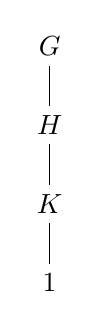
\begin{tikzpicture}
                %Nodes
                \node at (0,0) (G) {$G$};
                \node at (0,-1) (H) {$H$};
                \node at (0,-2) (K) {$K$};
                \node at (0,-3) (1) {$1$};
    
                %Lines
                \draw (1) -- (K);
                \draw (K) -- (H);
                \draw (H) -- (G);
            \end{tikzpicture}
        \end{center}

        \item If $H \leq K$, then it obviously follows that $H \cap K = H$ and $\langle H,K \rangle = K$. Therefore, the lattice can be drawn as follows:
        
        \begin{center}
            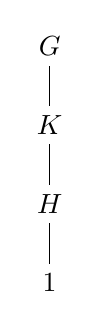
\begin{tikzpicture}
                %Nodes
                \node at (0,0) (G) {$G$};
                \node at (0,-1) (K) {$K$};
                \node at (0,-2) (H) {$H$};
                \node at (0,-3) (1) {$1$};
    
                %Lines
                \draw (1) -- (H);
                \draw (H) -- (K);
                \draw (K) -- (G);
            \end{tikzpicture}
        \end{center}

        \item If $H$ and $K$ are not comparable, all of $H$, $K$, $H\cap K$ and $\langle H,K \rangle$ are distinct. Hence:
        
        \begin{center}
            \begin{tikzpicture}
                %Nodes
                \node at (0,0)   (G)   {$G$};
                \node at (0,-1.5)(HUK) {$\langle H,K\rangle$};
                \node at (-2,-3) (H)   {$H$};
                \node at (2,-3)  (K)   {$K$};
                \node at (0,-4.5)(HAK){$H\cap K$};
                \node at (0,-6)  (1)   {$1$};
    
                %Lines
                \draw (1) -- (HAK);
                \draw (HAK) -- (H);
                \draw (HAK) -- (K);
                \draw (H) -- (HUK);
                \draw (K) -- (HUK);
                \draw (HUK) -- (G);
            \end{tikzpicture}
        \end{center}
    \end{enumerate}

    Therefore, the only thing that distinguishes the different drawings, beside the name of the nodes, is the fact that one is a straight line and the other splits in the middle. \\
\end{solution}

\begin{exercise}
    In each of (a) to (d) list all subgroups of $D_{16}$ that satisfy the given conition.
    \begin{enumerate}[label = \textbf{(\alph*)}]
        \item Subgroups that are contained in $\langle sr^2, r^4 \rangle$
        \item Subgroups that are contained in $\langle sr^7, r^4 \rangle$
        \item Subgroups that contain $\langle r^4 \rangle$
        \item Subgroups that contain $\langle s \rangle$.
    \end{enumerate}
\end{exercise}

\begin{solution}
    \begin{enumerate}[label = \textbf{(\alph*)}]
        \item The subgroups of $D_{16}$ that are contained in $\langle sr^2, r^4 \rangle$ are 
        $$1, \quad \langle sr^6\rangle, \quad \langle sr^2 \rangle, \quad \langle r^4 \rangle, \quad \langle sr^2, r^4 \rangle$$
        \item First, notice that $\langle sr^7, r^4 \rangle$ is equal to $\langle sr^3, r^4 \rangle$. Hence, the subgroups of $D_{16}$ that are contained in $\langle sr^7, r^4 \rangle$ are 
        $$1, \quad \langle sr^3\rangle, \quad \langle sr^7 \rangle, \quad \langle r^4 \rangle, \quad \langle sr^7, r^4 \rangle$$
        \item The subgroups of $D_{16}$ that contain $\langle r^4 \rangle$ are 
        $$\langle r^4 \rangle, \quad \langle sr^2, r^4\rangle, \quad \langle s, r^4\rangle, \quad \langle r^2\rangle, \quad \langle sr^3, r^4\rangle$$
        $$\langle sr^5, r^4\rangle, \quad \langle s, r^2\rangle, \quad \langle r \rangle, \quad \langle sr, r^2\rangle, \quad D_{16}$$
        \item The subgroups of $D_{16}$ that contain $\langle s \rangle$ are 
        $$\langle s \rangle, \quad \langle s, r^4\rangle, \quad \langle s, r^2\rangle, \quad D_{16}$$
    \end{enumerate}
\end{solution}

\begin{exercise}
    Show that the subgroup $\langle s, r^2\rangle$ of $D_8$ is isomorphic to $V_4$. \\
\end{exercise}

\begin{solution}
    \\ First, recall that $V_4 = \{1, a, b, c\}$ with the following multiplication table:

    \begin{table}[h!]
    \centering
    \begin{tabular}{l|l l l l}
    $\cdot$ & 1   & $a$ & $b$ & $c$ \\ \hline
    1       & 1   & $a$ & $b$ & $c$ \\ 
    $a$     & $a$ & 1   & $c$ & $b$ \\ 
    $b$     & $b$ & $c$ & 1   & $a$ \\ 
    $c$     & $c$ & $b$ & $a$ & 1  
    \end{tabular}
    \end{table}
    
    Notice that $\{1, s, r^2, sr^2\}$ is a group subgroup of $D_8$ that contains $s$, $r^2$ and all of the possible combinations of these elements. Hence,
    $$\langle s, r^2\rangle = \{1, s, r^2, sr^2\}$$
    From this, we get the following multiplication table for $\langle s, r^2\rangle$:

    \begin{table}[h!]
    \centering
    \begin{tabular}{l|l l l l}
    $\cdot$ & 1      & $s$    & $r^2$  & $sr^2$ \\ \hline
    1       & 1      & $s$    & $r^2$  & $sr^2$ \\ 
    $s$     & $s$    & 1      & $sr^2$ & $r^2$  \\ 
    $r^2$   & $r^2$  & $sr^2$ & 1      & $s$    \\ 
    $sr^2$  & $sr^2$ & $r^2$  & $s$    & 1  
    \end{tabular}
    \end{table}

    \break \noindent which directly implies that the function $\varphi : \langle s, r^2\rangle \to V_4$ defined by
    $$1 \mapsto 1, \quad a \mapsto s, \quad b \mapsto r^2, \quad c \mapsto sr^2$$
    is an isomorphism. Therefore, $\langle s, r^2\rangle \cong V_4$. \\
\end{solution}

\begin{exercise}
    Use the given lattice to find all pairs of elements that generate $D_8$ (there are 12 pairs). \\
\end{exercise}

\begin{solution}
    \\ Recall that the lattice of subgroups of $D_8$ looks like this:

    \begin{center}
        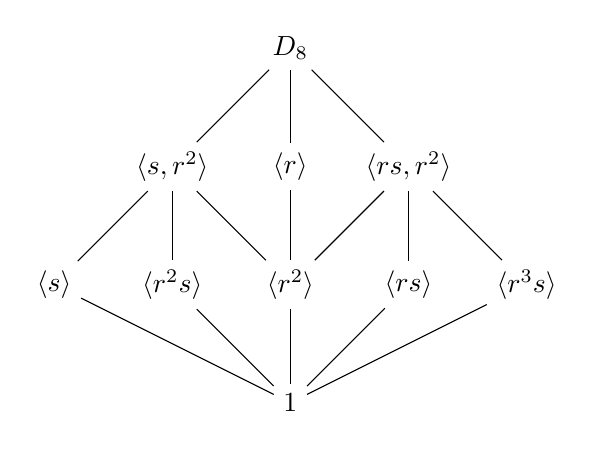
\begin{tikzpicture}
            %Nodes
            \node at (0,0)      (D8)  {$D_8$};
            \node at (0,-1.5)   (r)   {$\langle r \rangle$};
            \node at (-1.5,-1.5)(sr2){$\langle s,r^2\rangle$};
            \node at (1.5,-1.5) (rsr2){$\langle rs,r^2\rangle$};
            \node at (0,-3)     (r2)   {$\langle r^2 \rangle$};
            \node at (1.5,-3)   (rs)   {$\langle rs \rangle$};
            \node at (3,-3)     (r3s)  {$\langle r^3s \rangle$};
            \node at (-3,-3)    (s)  {$\langle s \rangle$};
            \node at (-1.5,-3)  (r2s) {$\langle r^2s \rangle$};
            \node at (0,-4.5)   (1){$1$};

            %Lines
            \draw (1)    -- (r2);
            \draw (1)    -- (r2s);
            \draw (1)    -- (s);
            \draw (1)    -- (rs);
            \draw (1)    -- (r3s);
            \draw (s)    -- (sr2);
            \draw (r2s)  -- (sr2);
            \draw (r2)   -- (sr2);
            \draw (r2)   -- (rsr2);
            \draw (rs)   -- (rsr2);
            \draw (r3s)  -- (rsr2);
            \draw (r2)   -- (r);
            \draw (sr2)  -- (D8);
            \draw (r)    -- (D8);
            \draw (rsr2) -- (D8);
        \end{tikzpicture}
    \end{center}
    Finding pairs $(a,b)$ such that $\langle a,b \rangle = D_8$ is equivalent to finding elements $a$ and $b$ such that the least common upperbound of their corresponding sets $\langle a \rangle$ and $\langle b \rangle$ on the lattice is $D_8$. Hence, if we recall that $\langle r^3 \rangle = \langle r \rangle$, then we get the following pairs:
    $$(s,r), \quad (s, rs), \quad (s,r^3s), \quad (r^2s,r), \quad (r^2s, rs), \quad (r^2s,r^3s)$$
    $$(s,r^3), \quad (r, rs), \quad (r,r^3s), \quad (r^2s,r^3), \quad (r^3, rs), \quad (r^3,r^3s)$$
    \break
\end{solution}

\begin{exercise}
    Use the given lattice to find all elements $x \in D_{16}$ such that $D_{14} = \langle x, s \rangle$ (there are 8 such elements). \\
\end{exercise}

\begin{solution}
    \\ The idea is exactly the same as for the previous exercise. Hence, our possible values for $x$ are:
    $$r, \quad r^3, \quad r^5, \quad r^7, \quad sr, \quad sr^3, \quad sr^5, \quad sr^7$$
\end{solution}

\begin{exercise}
    Use the given lattices to help find the centralizers of every element in the following groups:\\
    $\textbf{(a)} \ D_8 \qquad \textbf{(b)} \ Q_8 \qquad \textbf{(c)} \ S_3 \qquad \textbf{(d)} \ D_{16} $ \\
\end{exercise}

\begin{solution}
    \begin{enumerate}[label = \textbf{(\alph*)}]
        \item \begin{multicols}{3}\begin{itemize}
            \item $C_{D_8}(1) = D_8$
            \item $C_{D_8}(r) = \langle r \rangle$
            \item $C_{D_8}(r^2) = D_8$
            \item $C_{D_8}(r^3) = \langle r \rangle$
            \item $C_{D_8}(s) = \langle s, r^2 \rangle$
            \item $C_{D_8}(rs) = \langle rs, r^2 \rangle$
            \item $C_{D_8}(r^2s) = \langle s, r^2 \rangle$
            \item $C_{D_8}(r^3s) = \langle rs, r^2 \rangle$
        \end{itemize}
        \end{multicols}
        \item \begin{multicols}{3}\begin{itemize}
            \item $C_{Q_8}(1) = Q_8$
            \item $C_{Q_8}(-1) = Q_8$
            \item $C_{Q_8}(i) = \langle i \rangle$
            \item $C_{Q_8}(-i) = \langle i \rangle$
            \item $C_{Q_8}(j) = \langle j \rangle$
            \item $C_{Q_8}(-j) = \langle j \rangle$
            \item $C_{Q_8}(k) = \langle k \rangle$
            \item $C_{Q_8}(-k) = \langle k \rangle$
        \end{itemize}
        \end{multicols}
    \item \begin{multicols}{2}\begin{itemize}
            \item $C_{S_3}(1) = S_3$
            \item $C_{S_3}((1 \ 2)) = \langle (1 \ 2) \rangle$
            \item $C_{S_3}((1 \ 3)) = \langle (1 \ 3) \rangle$
            \item $C_{S_3}((2 \ 3)) = \langle (2 \ 3) \rangle$
            \item $C_{S_3}((1 \ 2 \ 3)) = \langle (1 \ 2 \ 3) \rangle$
            \item $C_{S_3}((1 \ 3 \ 2)) = \langle (1 \ 3 \ 2) \rangle$
        \end{itemize}
        \end{multicols}
    \item \begin{multicols}{2}\begin{itemize}
            \item $C_{D_{16}}(1) = D_{16}$
            \item $C_{D_{16}}(r) = \langle r \rangle$
            \item $C_{D_{16}}(r^2) = \langle r \rangle$
            \item $C_{D_{16}}(r^3) = \langle r \rangle$
            \item $C_{D_{16}}(r^4) = D_{16}$
            \item $C_{D_{16}}(r^5) = \langle r \rangle$
            \item $C_{D_{16}}(r^6) = \langle r \rangle$
            \item $C_{D_{16}}(r^7) = \langle r \rangle$
            \item $C_{D_{16}}(s) = \langle s, r^4 \rangle$
            \item $C_{D_{16}}(sr) = \langle sr^5, r^4 \rangle$
            \item $C_{D_{16}}(sr^2) = \langle sr^2, r^4 \rangle$
            \item $C_{D_{16}}(sr^3) = \langle sr^3, r^4 \rangle$
            \item $C_{D_{16}}(sr^4) = \langle s, r^4 \rangle$
            \item $C_{D_{16}}(sr^5) = \langle sr^5, r^4 \rangle$
            \item $C_{D_{16}}(sr^6) = \langle sr^2, r^4 \rangle$
            \item $C_{D_{16}}(sr^7) = \langle sr^3, r^4 \rangle$
        \end{itemize}
        \end{multicols}
    \end{enumerate}
\end{solution}

\begin{exercise}
    Find the center of $D_{16}$.\\
\end{exercise}

\begin{solution}
    \\ To find the center of $D_{16}$, we can take the intersection of all the subgroups we found in part (d) of the previous question, that is:
    $$D_{16}\cap \langle r \rangle \cap \langle s, r^4 \rangle \cap \langle sr^2, r^4 \rangle \cap \langle sr^3, r^4 \rangle \cap \langle sr^5, r^4 \rangle$$
    Obviously, 1 and $r^4$ are in this intersection. However, since $sr^i \notin \langle r \rangle$ for $i \in \Iint{0}{n-1}$, then other elements in the intersection must be powers of $r$. However, the only power of $r$ in $\langle s, r^4 \rangle$ is $r^4$. Therefore,
    $$Z(D_{16}) = \{1, r^4\}$$
\end{solution}

\begin{exercise}
    In each of the following groups find the normalizer of each subgroup:\\
    $\textbf{(a)} \ S_3 \qquad \textbf{(b)} \ Q_8$ \\
\end{exercise}

\begin{solution}
    \begin{enumerate}[label = \textbf{(\alph*)}]
        \item \begin{multicols}{2}\begin{itemize}
            \item $N_{S_3}(1) = S_3$
            \item $N_{S_3}(\langle (1 \ 2) \rangle) = \langle (1 \ 2) \rangle$
            \item $N_{S_3}(\langle (1 \ 3) \rangle) = \langle (1 \ 3) \rangle$
            \item $N_{S_3}(\langle (2 \ 3) \rangle) = \langle (2 \ 3) \rangle$
            \item $N_{S_3}(\langle (1 \ 2 \ 3) \rangle) = S_3$
            \item $N_{S_3}(S_3) = S_3$
        \end{itemize}
        \end{multicols}
        \item \begin{multicols}{2}\begin{itemize}
            \item $N_{Q_8}(1) = Q_8$
            \item $N_{Q_8}(\langle -1 \rangle) = Q_8$
            \item $N_{Q_8}(\langle i \rangle) = Q_8$
            \item $N_{Q_8}(\langle j \rangle) = Q_8$
            \item $N_{Q_8}(\langle k \rangle) = Q_8$
            \item $N_{Q_8}(Q_8) = Q_8$
        \end{itemize}
        \end{multicols}
    \end{enumerate}
\end{solution}

\begin{exercise}
    Draw the lattices of subrgoups of the following groups:\\
    $\textbf{(a)} \ \Z{16} \qquad \textbf{(b)} \ \Z{24} \qquad \textbf{(c)} \ \Z{48}. \ $ [See Exercise 6 in Section 3.]\\ 
\end{exercise}

\begin{solution}
    \begin{enumerate}[label = \textbf{(\alph*)}]
        \item Lattice of subgroups of $\Z{16}$:
            \begin{center}
            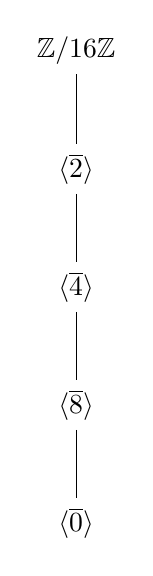
\begin{tikzpicture}
                %Nodes
                \node at (0,0)      (1)  {$\Z{16}$};
                \node at (0,-1.5)   (2)  {$\langle \overline{2} \rangle$};
                \node at (0,-3)     (4)  {$\langle \overline{4} \rangle$};
                \node at (0,-4.5)   (8)  {$\langle \overline{8} \rangle$};
                \node at (0,-6)     (0) {$\langle \overline{0} \rangle$};
    
    
                %Lines
                \draw (1) -- (2);
                \draw (2) -- (4);
                \draw (4) -- (8);
                \draw (8) -- (0);
            \end{tikzpicture}
            \end{center}
        \item Lattice of subgroups of $\Z{24}$:
            \begin{center}
            \begin{tikzpicture}
                %Nodes
                \node at (1.5,0)   (1)  {$\Z{24}$};
                \node at (0,-1.5)  (3)  {$\langle \overline{3} \rangle$};
                \node at (3,-1.5)  (2)  {$\langle \overline{2} \rangle$};
                \node at (1.5,-3)  (6)  {$\langle \overline{6} \rangle$};
                \node at (4.5,-3)  (4)  {$\langle \overline{4} \rangle$};
                \node at (3,-4.5)  (12) {$\langle \overline{12} \rangle$};
                \node at (6,-4.5)  (8)  {$\langle \overline{8} \rangle$};
                \node at (4.5,-6)  (0) {$\langle \overline{0} \rangle$};
    
    
                %Lines
                \draw (1) -- (3);
                \draw (1) -- (2);
                \draw (6) -- (2);
                \draw (3) -- (6);
                \draw (6) -- (12);
                \draw (2) -- (4);
                \draw (4) -- (12);
                \draw (12) -- (0);
                \draw (4) -- (8);
                \draw (8) -- (0);
            \end{tikzpicture}
            \end{center}
        \item We already drew the lattice of subgroups of $\Z{48}$ in Exercise 6 of section 3:
        \begin{center}
            \begin{tikzpicture}
                %Nodes
                \node at (1.5,0)   (1)  {$\mathbb{Z}/48\mathbb{Z}$};
                \node at (0,-1.5)  (3)  {$\langle \overline{3} \rangle$};
                \node at (3,-1.5)  (2)  {$\langle \overline{2} \rangle$};
                \node at (1.5,-3)  (6)  {$\langle \overline{6} \rangle$};
                \node at (4.5,-3)  (4)  {$\langle \overline{4} \rangle$};
                \node at (3,-4.5)  (12) {$\langle \overline{12} \rangle$};
                \node at (6,-4.5)  (8)  {$\langle \overline{8} \rangle$};
                \node at (4.5,-6)  (24) {$\langle \overline{24} \rangle$};
                \node at (7.5,-6)  (16) {$\langle \overline{16} \rangle$};
                \node at (6,-7.5)  (0)  {$\langle \overline{0} \rangle$};
    
    
                %Lines
                \draw (1) -- (3);
                \draw (1) -- (2);
                \draw (6) -- (2);
                \draw (3) -- (6);
                \draw (6) -- (12);
                \draw (2) -- (4);
                \draw (4) -- (12);
                \draw (12) -- (24);
                \draw (4) -- (8);
                \draw (8) -- (24);
                \draw (0) -- (24);
                \draw (8) -- (16);
                \draw (0) -- (16);
            \end{tikzpicture}
        \end{center}
    \end{enumerate}
\end{solution}

\begin{exercise}
    Classify groups of order 4 by proving that if $|G|=4$ then $G \cong Z_4$ or $G \cong V_4$. [See Exercise 36, Section 1.1.] \\
\end{exercise}

\begin{solution}
    \\ Let's prove it by cases. If $G$ contains an element of order 4, then it directly follows that $G$ is a cyclic group of order 4 which implies that $G \cong Z_4$. \\
    Otherwise, if $G$ has no elements of order 4, then we already proved in Exercise 36 of Section 1.1 that it automoaticaly implies that $G$ has the following multiplication table:
    \begin{table}[h!]
        \centering
        \begin{tabular}{l|l l l l}
        $\cdot$ & 1   & $a$ & $b$ & $c$ \\ \hline
        1       & 1   & $a$ & $b$ & $c$ \\ 
        $a$     & $a$ & 1   & $c$ & $b$ \\ 
        $b$     & $b$ & $c$ & 1   & $a$ \\ 
        $c$     & $c$ & $b$ & $a$ & 1  
        \end{tabular}
    \end{table}
    which is exactly the same multiplication as $V_4$ so both are isomorphic. Therefore, we either have $G \cong Z_4$ or $G \cong V_4$. \\
\end{solution}

\begin{exercise}
    Consider the group of order 16 with the following presentation:
    $$QD_{16} = \langle \ \sigma, \tau \ | \ \sigma^8 = \tau^2 = 1, \ \sigma\tau = \tau\sigma^3 \ \rangle$$
    (called the \textit{quasidihedral} or \textit{semidihedral} group of order 16). This group has three subgroups of order 8: $\langle \tau, \sigma^2 \rangle \cong D_8$, $\langle \tau \rangle \cong Z_8$ and $\langle \sigma^2, \sigma\tau \rangle \cong Q_8$ and every proper subgroup is contained in one of these subgroups. Fill in the missing subgroups in the lattice of all subgroups of the quasidihedral group on the following page, exhibiting each subgroup with at most two generators. (This is another example of a nonplanar lattice.) \\
\end{exercise}

\begin{solution}
    \\ Using the isomorphisms $\langle \tau, \sigma^2 \rangle \cong D_8$, $\langle \tau \rangle \cong Z_8$ and $\langle \sigma^2, \sigma\tau \rangle \cong Q_8$, we can make our life easier by considering $\sigma^2$ and $\tau$ as $r$ and $s$ respectively in $D_8$. Moreover, in the same way, we can consider $\sigma^4$, $\sigma^2$, $\tau\sigma$ and $\tau\sigma^7$ as -1, $i$, $j$ and $k$ respectively. Therefore, we get the following lattice of subgroups for $QD_{16}$:
    \begin{center}
        \begin{tikzpicture}
            %Nodes
            \node at (0,0)   (16)    {$QD_{16}$};
            \node at (-3,-2.5) (s2t)  {$\langle \sigma^2, \tau \rangle$}; 
            \node at (0,-2.5)  (s)    {$\langle \sigma \rangle$}; 
            \node at (3,-2.5) (s2ts)  {$\langle \sigma^2, \tau\sigma \rangle$};
            \node at (-6,-5)  (s2ts4) {$\langle \sigma^2\tau, \sigma^4 \rangle$};
            \node at (-3,-5)  (s4t) {$\langle \sigma^4, \tau \rangle$}; 
            \node at (0,-5)   (s2)  {$\langle \sigma^2 \rangle$};
            \node at (3,-5)   (ts)  {$\langle \tau \sigma \rangle$};
            \node at (6,-5)   (ts7)  {$\langle \tau \sigma^7 \rangle$};
            \node at (-7,-7.5) (ts2)  {$\langle \tau \sigma^2 \rangle$};
            \node at (-5,-7.5) (s2th)  {$\langle \sigma^2 \tau\rangle$};
            \node at (-3.5,-7.5) (s4th)  {$\langle \sigma^4 \tau\rangle$};
            \node at (-2,-7.5) (t)  {$\langle \tau \rangle$};
            \node at (0,-7.5) (s4)  {$\langle \sigma^4 \rangle$};
            \node at (0,-10) (1)  {1};
            \node (i) at (intersection of s4--s2ts4 and s4t--s4th) {}; 
            \node (ii) at (intersection of s4--s2ts4 and s4t--t) {}; 

            %Lines
            \draw (16) -- (s2t);
            \draw (16) -- (s);
            \draw (16) -- (s2ts);
            \draw (s2t) -- (s2ts4);
            \draw (s2t) -- (s4t);
            \draw (s2t) -- (s2);
            \draw (s) -- (s2);
            \draw (s2ts) -- (s2);
            \draw (s2ts) -- (ts);
            \draw (s2ts) -- (ts7);
            \draw (ts2) -- (s2ts4);
            \draw (s2th) -- (s2ts4);
            \draw (s4th) -- (i);
            \draw (i) -- (s4t);
            \draw (t) -- (ii);
            \draw (ii) -- (s4t);
            \draw (s4) -- (s4t);
            \draw (s4) -- (s2);
            \draw (s4) -- (ts);
            \draw (s4) -- (ts7);
            \draw (s4) -- (s2ts4);
            \draw (1) -- (ts2);
            \draw (1) -- (s2th);
            \draw (1) -- (s4th);
            \draw (1) -- (t);
            \draw (1) -- (s4);
        \end{tikzpicture}
    \end{center}
\end{solution}

\begin{exercise}
    The group $A = Z_2 \times Z_4 = \langle \ a,b \ | a^2 = b^4 = 1, \ ab = ba \ \rangle$ has order 8 and has three subgroups of order 4: $\langle a, b^2 \rangle \cong V_4$, $\langle b \rangle \cong Z_4$ and $\langle a b \rangle \cong Z_4$ and every proper subgroup is contained in one of these three. Draw the lattice of all subgroups of $A$, giving each subgroup in terms of at most two generators. \\
\end{exercise}

\begin{solution}
    As in the previous exercise, we will mostly rely on the fact that all the subgroups of order 4 are $\langle a, b^2 \rangle \cong V_4$, $\langle b \rangle \cong Z_4$ and $\langle a b \rangle \cong Z_4$. Hence, we get:
    \begin{center}
        \begin{tikzpicture}
            %Nodes
            \node at (0,0)   (A)    {$A$};
            \node at (-3,-2) (ab2)  {$\langle a,b^2\rangle$}; 
            \node at (0,-2)  (b)    {$\langle b \rangle$}; 
            \node at (3,-2)  (ab)   {$\langle ab \rangle$};
            \node at (-6,-4) (a)    {$\langle a \rangle$};
            \node at (-3,-4) (ab2h) {$\langle ab^2 \rangle$}; 
            \node at (0,-4)  (b2)   {$\langle b^2 \rangle$};
            \node at (0,-6)  (1)    {$ 1 $};

            %Lines
            \draw (A) -- (ab2);
            \draw (A) -- (b);
            \draw (A) -- (ab);
            \draw (a) -- (ab2);
            \draw (ab2h) -- (ab2);
            \draw (b2) -- (ab2);
            \draw (b2) -- (b);
            \draw (b2) -- (ab);
            \draw (a) -- (1);
            \draw (ab2h) -- (1);
            \draw (b2) -- (1);
        \end{tikzpicture}
    \end{center}
\end{solution}

\begin{exercise}
    The group $G = Z_2 \times Z_8 = \langle \ x,y \ | x^2 = y^8 = 1, \ xy = yx \ \rangle$ has order 16 and has three subgroups of order 8: $\langle x, y^2 \rangle \cong Z_2\times Z_4$, $\langle y \rangle \cong Z_8$ and $\langle xy \rangle \cong Z_8$ and every proper subgroup is contained in one of these three. Draw the lattice of all subgroups of $G$, giving each subgroup in terms of at most two generators (cf. Exercise 12 ). \\
\end{exercise}

\begin{solution}
    As in the previous exercise, we will mostly rely on the fact that all the subgroups of order 8 are $\langle x, y^2 \rangle \cong Z_2\times Z_4$, $\langle y \rangle \cong Z_8$ and $\langle xy \rangle \cong Z_8$. Moreover, since we already drew the lattice of subgroups of the group $Z_2 \times Z_4$ in the previous question, then we get:
    \begin{center}
        \begin{tikzpicture}
            %Nodes
            \node at (0,0)   (G)    {$G$};
            \node at (-3,-2) (y)   {$\langle y \rangle$}; 
            \node at (0,-2)  (xy)    {$\langle xy \rangle$}; 
            \node at (3,-2)  (xvy2) {$\langle x,y^2 \rangle$};
            \node at (0,-4) (y2)   {$\langle y^2 \rangle$}; 
            \node at (3,-4)  (xy2)  {$\langle xy^2 \rangle$};
            \node at (6,-4)  (xvy4) {$\langle x,y^4 \rangle$};
            \node at (3,-6) (y4)   {$\langle y^4 \rangle$}; 
            \node at (6,-6)  (x)    {$\langle x \rangle$};
            \node at (9,-6)  (xy4)  {$\langle xy^4 \rangle$};
            \node (i) at (intersection of y4--xvy4 and x--xy2) {}; 
            \node at (6,-8)  (1)    {$ 1 $};

            %Lines
            \draw (G) -- (xy);
            \draw (G) -- (y);
            \draw (G) -- (xvy2);
            \draw (y2) -- (xy);
            \draw (y2) -- (y);
            \draw (y2) -- (xvy2);
            \draw (xy2) -- (xvy2);
            \draw (xvy4) -- (xvy2);
            \draw (y4) -- (y2);
            \draw (y4) -- (xy2);
            \draw (y4) -- (i);
            \draw (i) -- (xvy4);
            \draw (x) -- (xy2);
            \draw (xy4) -- (xvy4);
            \draw (y4) -- (1);
            \draw (x) -- (1);
            \draw (x) -- (xvy4);
            \draw (xy4) -- (1);
        \end{tikzpicture}
    \end{center}
\end{solution}

\begin{exercise}
    Let $M$ be the group of order 16 with the following presentation:
    $$\langle \ u,v \ | \ u^2 = v^8 = 1, \ vu = uv^5 \ \rangle$$
    (sometimes called the \textit{modular} group of order 16). It has three subgroups of order 8: $\langle u,v^2 \rangle$, $\langle v \rangle$ and $\langle uv \rangle$ and every proper subgroup is contained in oneof these three. Prove that $\langle u, v^2 \rangle \cong Z_2\times Z_4$, $\langle v \rangle \cong Z_8$ and $\langle uv \rangle \cong Z_8$. Show that the lattice of subgroups of $M$ is the same as the lattice of subgroups of $Z_2 \times Z_8$ (cf. Exercise 13) but that these two groups are not isomorphic. \\
\end{exercise}

\begin{solution}
    \\ First, let's prove the three isomorphisms. Obviously, $\langle v \rangle \cong Z_8$ since $v$ is an element of order 8. Similarly, to show that $\langle uv \rangle \cong Z_8$, we simply need to show that $uv$ has order 8. To do so, notice that 
    $$(uv)^2 = uvuv = uuv^5v = v^6$$
    Thus,
    $$(uv)^8 = (v^6)^4 = v^{24} = 1$$
    Hence, $uv$ must have order 1, 2, 4 or 8. But notice that
    $$(uv)^4 = (v^6)^2 = v^12 = v^4 \neq 1$$
    Therefore, $uv$ has order 8 which shows that $\langle uv \rangle \cong Z_8$. Finally, since
    $$uv^2 = (uv^2)v^8 = (uv^5)v^5 = v(uv^5) = v^2u$$
    then elements in $\langle u, v^2 \rangle$ have the form $u^n(v^2)^m$. Thus, obviously, $\langle u, v^2 \rangle \cong Z_2\times Z_4$. From this, we get that
    \begin{center}
        \begin{tikzpicture}
            %Nodes
            \node at (0,0)   (G)    {$G$};
            \node at (-3,-2) (y)   {$\langle v \rangle$}; 
            \node at (0,-2)  (xy)    {$\langle uv \rangle$}; 
            \node at (3,-2)  (xvy2) {$\langle u,v^2 \rangle$};
            \node at (0,-4) (y2)   {$\langle v^2 \rangle$}; 
            \node at (3,-4)  (xy2)  {$\langle uv^2 \rangle$};
            \node at (6,-4)  (xvy4) {$\langle u,v^4 \rangle$};
            \node at (3,-6) (y4)   {$\langle v^4 \rangle$}; 
            \node at (6,-6)  (x)    {$\langle u \rangle$};
            \node at (9,-6)  (xy4)  {$\langle uv^4 \rangle$};
            \node (i) at (intersection of y4--xvy4 and x--xy2) {}; 
            \node at (6,-8)  (1)    {$ 1 $};

            %Lines
            \draw (G) -- (xy);
            \draw (G) -- (y);
            \draw (G) -- (xvy2);
            \draw (y2) -- (xy);
            \draw (y2) -- (y);
            \draw (y2) -- (xvy2);
            \draw (xy2) -- (xvy2);
            \draw (xvy4) -- (xvy2);
            \draw (y4) -- (y2);
            \draw (y4) -- (xy2);
            \draw (y4) -- (i);
            \draw (i) -- (xvy4);
            \draw (x) -- (xy2);
            \draw (xy4) -- (xvy4);
            \draw (y4) -- (1);
            \draw (x) -- (1);
            \draw (x) -- (xvy4);
            \draw (xy4) -- (1);
        \end{tikzpicture}
    \end{center}
    which obviously shows that $M$ has the same lattice of subgroups of $Z_2 \times Z_8$.\\
    Now, let's show that $M \not\cong Z_2 \times Z_8$. By contradiction, if $M \cong Z_2 \times Z_8$, then $M$ must be abelian so we have 
    $$uv = vu = uv^5$$
    which implies that 
    $$v^4 = 1$$
    But this is a contradiction since $v$ has order 8. Therefore, $M \not\cong Z_2 \times Z_8$ even if they have the same lattice of subgroups. \\
\end{solution}

\begin{exercise}
    Describe the isomorphism type of each of the three subgroups of $D_{16}$ of order 8. \\
\end{exercise}

\begin{solution}
    The three subgroups of order 8 of $D_{16}$ are $\langle s, r^2 \rangle$, $\langle r \rangle$ and $\langle sr, r^2 \rangle$. Obviously, $\langle r \rangle \cong Z_8$ since it is cyclic and has order 8. By looking at the lattice of subgroups of $D_{16}$ and $D_8$, we can guess that both $\langle s, r^2 \rangle$ and $\langle sr, r^2 \rangle$ are isomorphic to $D_8$. To prove it, notice that the function that associates $s$ in $D_{16}$ to $s$ in $D_8$ and $r^2$ in $D_{16}$ to $r$ in $D_8$ extends to an isomorphism since $s$ has order 2, $r^2$ has order 4 and 
    $$(r^2)s = r(rs) = (rs)r^{-1} = s(r^2)^{-1}$$
    The same holds if we replace $s$ with $sr$. Therefore, we get that $\langle s, r^2 \rangle \cong \langle sr, r^2 \rangle \cong D_8$. \\
\end{solution}

\begin{exercise}
    Use the lattice of subgroups of the quasidihedral group of order 16 to show that every element of order 2 is contained in the proper subgroup $\langle \tau, \sigma^2 \rangle$ (cf. Exercise 11). \\
\end{exercise}

\begin{solution}
    \\ Proving this is equivalent to showing that every subgroup of $QD_{16}$ of order 2 is a subgroup of $\langle \tau, \sigma^2 \rangle$. The subgroups of order 2 are precisely $\langle \tau \rangle$, $\langle \sigma^4 \rangle$, $\langle \sigma^4\tau \rangle$, $\langle \sigma^2\tau \rangle$ and $\langle \tau\sigma^2 \rangle$. But notice that all of them are \textit{below} $\langle \tau, \sigma^2 \rangle$ in the lattice. Thus, $\langle \tau, \sigma^2 \rangle$ contains every element of order 2. \\
\end{solution}

\begin{exercise}
    Use the lattice of subgroups of the modular group $M$ of order 16 to show that the set $\{x\in M \ | \ x^2 = 1\}$ is a subgroup of $M$ isomorphic to the Klein 4-group (cf. Exercise 14). \\
\end{exercise}

\begin{solution}
    \\ The elements $x$ in $M$ that satisfy $x^2 = 1$ are precisely 1, $v^4$, $u$ and $uv^4$. But notice that $\langle u, v^4 \rangle$ contains exactly these four elements. Hence, it is a subgroup of $M$ of order 4 that is not cyclic, thus, it must isomorphic the Klein 4-group. \\ 
\end{solution}

\begin{exercise}
    Use the lattice to help find the centralizers of every element of $QD_{16}$ (cf. Exercise 11). \\
\end{exercise}

\begin{solution}
    \begin{multicols}{2}\begin{itemize}
        \item $C_{QD_{16}}(1) = QD_{16}$
        \item $C_{QD_{16}}(\sigma) = \langle \sigma \rangle$
        \item $C_{QD_{16}}(\sigma^2) = \langle \sigma \rangle$
        \item $C_{QD_{16}}(\sigma^3) = \langle \sigma \rangle$
        \item $C_{QD_{16}}(\sigma^4) = QD_{16}$
        \item $C_{QD_{16}}(\sigma^5) = \langle \sigma \rangle$
        \item $C_{QD_{16}}(\sigma^6) = \langle \sigma \rangle$
        \item $C_{QD_{16}}(\sigma^7) = \langle \sigma \rangle$
        \item $C_{QD_{16}}(\tau) = \langle \sigma^4, \tau \rangle$
        \item $C_{QD_{16}}(\tau\sigma) = \langle \tau\sigma \rangle$
        \item $C_{QD_{16}}(\tau\sigma^2) = \langle \sigma^2\tau, \sigma^4 \rangle$
        \item $C_{QD_{16}}(\tau\sigma^3) = \langle \tau \sigma^7 \rangle$
        \item $C_{QD_{16}}(\tau\sigma^4) = \langle \sigma^4, \tau \rangle$
        \item $C_{QD_{16}}(\tau\sigma^5) = \langle \tau\sigma \rangle$
        \item $C_{QD_{16}}(\tau\sigma^6) = \langle \sigma^2\tau, \sigma^4 \rangle$
        \item $C_{QD_{16}}(\tau\sigma^7) = \langle \tau\sigma^7 \rangle$
    \end{itemize}
    \end{multicols}
\end{solution}

\begin{exercise}
    Use the lattice to help find $N_{D_{16}}(\langle s, r^4 \rangle)$.\\
\end{exercise}

\begin{solution}
    \\ To find the normalizer of $\langle s, r^4 \rangle$, first notice that 
    \begin{align*}
        s\langle s, r^4 \rangle s^{-1} &= \{s1s, \ sss, \ sr^4s, \ ssr^4s\} \\
        &= \{1, \ s, \ r^4, \ sr^4\} \\
        &= \langle s, r^4 \rangle
    \end{align*}
    and 
    \begin{align*}
        r^2\langle s, r^4 \rangle r^{-2} &= \{r^2 1r^{-2}, \ r^2 sr^{-2}, \ r^2 r^4 r^{-2}, \ r^2 sr^4 r^{-2}\} \\
        &= \{1, \ sr^4, \ r^4, \ s\} \\
        &= \langle s, r^4 \rangle
    \end{align*}
    which implies that both $s$ and $r^2$ are in $N_{D_{16}}(\langle s, r^4 \rangle)$. Thus, $\langle s, r^2 \rangle \leq N_{D_{16}}(\langle s, r^4 \rangle)$ which implies by the given lattice that $N_{D_{16}}(\langle s, r^4 \rangle)$ is either $\langle s, r^2 \rangle$ or $D_{16}$. However, notice that 
    \begin{align*}
        r\langle s, r^4 \rangle r^{-1} &= \{r 1 r^{-1}, \ r sr^{-1}, \ r r^4 r^{-1}, \ r sr^4 r^{-1}\} \\
        &= \{1, \ sr^6, \ r^4, \ sr^2\} \\
        &\neq \langle s, r^4 \rangle
    \end{align*}
    so $N_{D_{16}}(\langle s, r^4 \rangle) \neq D_{16}$. Therefore, it follows that $N_{D_{16}}(\langle s, r^4 \rangle) = \langle s, r^2 \rangle$. \\ 
\end{solution}

\begin{exercise}
    Use the lattice of subgroups of $QD_{16}$ (cf. Exercise 11) to help find the normalizers \\
    $\textbf{(a)} \ N_{QD_{16}}(\langle \tau\sigma \rangle) \qquad \textbf{(b)} \ N_{QD_{16}}(\langle \tau, \sigma^4 \rangle)$ \\
\end{exercise}

\begin{solution}
    \begin{enumerate}[label = \textbf{(\alph*)}]
        \item To find the normalizer of $\langle \tau\sigma \rangle$, first notice that $\tau\sigma$ is obviously in it and that
        \begin{align*}
            \sigma^2\langle \tau\sigma \rangle \sigma^{-2} &= \{\sigma^2 1 \sigma^{-2}, \ \sigma^2 \tau\sigma \sigma^{-2}, \ \sigma^2 \sigma^4 \sigma^{-2}, \ \sigma^2 \tau\sigma^5 \sigma^{-2}\} \\
            &= \{1, \ \tau\sigma^5, \ \sigma^4, \ \tau\sigma\} \\
            &= \langle \tau\sigma \rangle
        \end{align*}
        which implies that both $\sigma^2$ and $\tau\sigma$ are in $N_{QD_{16}}(\langle \tau\sigma \rangle)$. Thus, $\langle \sigma^2, \tau\sigma \rangle \leq N_{QD_{16}}(\langle \tau\sigma \rangle)$ which implies by the given lattice that $N_{QD_{16}}(\langle \tau\sigma \rangle)$ is either $\langle \sigma^2, \tau\sigma \rangle$ or $QD_{16}$. However, notice that 
        \begin{align*}
            \sigma\langle \tau\sigma \rangle \sigma^{-1} &= \{\sigma 1 \sigma^{-1}, \ \sigma \tau\sigma \sigma^{-1}, \ \sigma \sigma^4 \sigma^{-1}, \ \sigma \tau\sigma^5 \sigma^{-1}\} \\
            &= \{1, \ \tau\sigma^3, \ \sigma^4, \ \tau\sigma^7\} \\
            &\neq \langle \tau\sigma \rangle
        \end{align*}
        so $N_{QD_{16}}(\langle \tau\sigma \rangle) \neq QD_{16}$. Therefore, it follows that $N_{QD_{16}}(\langle \tau\sigma \rangle) = \langle \sigma^2, \tau\sigma \rangle$.

        \item To find the normalizer of $\langle \tau, \sigma^4 \rangle$, first notice that
        \begin{align*}
            \sigma^2\langle \tau, \sigma^4 \rangle \sigma^{-2} &= \{\sigma^2 1 \sigma^{-2}, \ \sigma^2 \tau \sigma^{-2}, \ \sigma^2 \sigma^4 \sigma^{-2}, \ \sigma^2 \tau\sigma^4 \sigma^{-2}\} \\
            &= \{1, \ \tau\sigma^4, \ \sigma^4, \ \tau\sigma^4\} \\
            &= \langle \tau, \sigma^4 \rangle
        \end{align*}
        and 
        \begin{align*}
            \tau\langle \tau, \sigma^4 \rangle \tau^{-1} &= \{\tau 1 \tau^{-1}, \ \tau \tau \tau^{-1}, \ \tau \sigma^4 \tau^{-1}, \ \tau \tau\sigma^4 \tau^{-1}\} \\
            &= \{1, \ \tau, \ \sigma^4, \ \tau\sigma^4\} \\
            &= \langle \tau, \sigma^4 \rangle
        \end{align*}
        which implies that both $\sigma^2$ and $\tau$ are in $N_{QD_{16}}(\langle \tau, \sigma^4 \rangle)$. Thus, $\langle \sigma^2, \tau \rangle \leq N_{QD_{16}}(\langle \tau, \sigma^4 \rangle)$ which implies by the given lattice that $N_{QD_{16}}(\langle \tau\sigma \rangle)$ is either $\langle \sigma^2, \tau \rangle$ or $QD_{16}$. However, notice that 
        \begin{align*}
            \sigma\langle \tau, \sigma^4 \rangle \sigma^{-1} &= \{\sigma 1 \sigma^{-1}, \ \sigma \tau \sigma^{-1}, \ \sigma \sigma^4 \sigma^{-1}, \ \sigma \tau\sigma^4 \sigma^{-1}\} \\
            &= \{1, \ \tau\sigma^2, \ \sigma^4, \ \tau\sigma^6\} \\
            &\neq \langle \tau, \sigma^4 \rangle
        \end{align*}
        so $N_{QD_{16}}(\langle \tau, \sigma^4 \rangle) \neq QD_{16}$. Therefore, it follows that $N_{QD_{16}}(\langle \tau, \sigma^4 \rangle) = \langle \sigma^2, \tau \rangle$. \\ 
    \end{enumerate}
\end{solution}

% CHAPTER 1
\chapter{Quotient Groups and Homomorphisms}

\section{Definitions and Examples}

\begin{exercise}
    Let $\varphi : G \to H$ be a homomorphism and let $E$ be a subgroup of $H$. Prove that $\varphi^{-1}(E) \leq G$ (i.e., the preimage or pullback of a subgroup under a homomorphism is a subgroup). If $E \trianglelefteq H$ prove that $\varphi^{-1}(E) \trianglelefteq G$. Deduce that $\ker \varphi \trianglelefteq G$. \\
\end{exercise}

\begin{solution}
    \\ Let $E$ be a subgroup, to show that $\varphi^{-1}(E) \leq G$, we can use the subgroup criterion which says that if it is closed under $(x,y) \mapsto xy^{-1}$ then it is a subgroup. Let $x$ and $y$ be arbitrary elements of $\varphi^{-1}(E)$, then both $\varphi(x)$ and $\varphi(y)$ are in $E$. Thus, since $E$ is a subgroup of $H$, we have:
    \begin{align*}
        \varphi(x)\varphi(y)^{-1} \in E &\implies \varphi(xy^{-1}) \in E \\
        &\implies xy^{-1} \in \varphi^{-1}(E) 
    \end{align*}
    which lets us conclude that it is a subgroup.\\
    Suppose now that $E \trianglelefteq H$, then by the previous proof, we know that $\varphi^{-1}(E) \leq G$. Moreover, by Theorem 6, we have that for all $h \in H$, 
    $$h E h^{-1} \subseteq E$$
    Let $g$ be an arbitrary element in $G$, then for all $y\in g \varphi^{-1}(E) g^{-1}$, there is a $x \in \varphi^{-1}(E)$ such that $y = gxg^{-1}$. Thus,
    $$\varphi(y) = \varphi(g)\varphi(x)\varphi(g)^{-1} \in \varphi(g) E \varphi(g)^{-1} \subseteq E$$
    so $y\in \varphi^{-1}(E)$. Since it holds for all $y$, then $g \varphi^{-1}(E) g^{-1} \subseteq \varphi^{-1}(E)$. Therefore, since it holds for all $g \in G$, we get by Theorem 6: $\varphi^{-1}(E) \trianglelefteq G$. \\
    Trivialy, since $\{1\}$ is normal in $H$, then $\ker \varphi = \varphi^{-1}(\{1\})$ is normal in $G$.\\
\end{solution}

\begin{exercise}
    Let $\varphi : G \to H$ be a homomorphism of groups with kernel $K$ and let $a,b \in \varphi(G)$. Let $X \in G/K$ be the fiber above $a$ and let $Y$ be the fiber above $b$, i.e., $X = \varphi^{-1}(a)$, $Y = \varphi^{-1}(b)$. Fix an element $u$ of $X$ (so $\varphi(u) = a$). Prove that if $XY = Z$ in the quotient group $G/K$ and $w$ is any member of $Z$, then there is some $v \in Y$ such that $uv = w$. [Show $u^{-1}w \in Y$.] \\
\end{exercise}

\begin{solution}
    By the definition of the products of fibers, the set $XY$ is the fiber above $ab$. Hence:
    \begin{align*}
        w \in XY &\implies \varphi(w) = ab \\
        &\implies \varphi(w) = \varphi(u)b \\
        &\implies \varphi(u^{-1}w) = b \\
        &\implies u^{-1}w \in Y \\
        &\implies v = u^{-1}w, \qquad \text{for some }v\in Y\\
        &\implies uv = w, \qquad \text{for some }v\in Y\\
    \end{align*}
    which is the desired equality. \\
\end{solution}

\begin{exercise}
    Let $A$ be an abelian group and let $B$ be a subgroup of $A$. Prove that $A/B$ is abelian. Give an example of a non-abelian group $G$ containing a proper normal subgroup $N$ such that $G/N$ is abelian. \\
\end{exercise}

\begin{solution}
    \\ First, notice that $B$ must be normal since for all $a \in A$:
    $$a B = \{ab \ | \ b \in B\} = \{ba \ | \ b \in B\} = Ba$$
    Hence, $A/B$ is a group. Moreover, for all $uB, vB \in A/B$:
    $$(uB)(vB) = (uv)B = (vu)B = (vB)(uB)$$
    Therefore, $A/B$ is an abelian group. \\
    As an example of abelian group $G/N$ where $G$ is non-abelian and $N$ is a proper subgroup, take $G = D_8$ and $N = \langle r^2 \rangle$ and notice that $N$ must be normal since $N = Z(D_8)$. Moreover, $G/N$ contains the elements 
    $$\{1, r^2\}, \ \{r, r^3\}, \ \{s, sr^2\}, \ \{sr, sr^3\}$$
    hence it is a group of order 4. Therefore, by the classification of groups of order 4, $G/N$ must be abelian. \\ 
\end{solution}

\begin{exercise}
    Prove that in the quotient group $G/N$, $(gN)^{\alpha} = g^{\alpha}N$ for all $\alpha \in \mathbb{Z}$. \\
\end{exercise}

\begin{solution}
    \\ First, recall that $\phi : G \to G/N$ defined by $g \mapsto gN$ is a homomorphism. Hence, for all $\alpha \in \mathbb{Z}$, we have:
    $$\phi(g^{\alpha}) = \varphi(g)^{\alpha}$$
    which is equivalent to
    $$(gN)^{\alpha} = g^{\alpha}N$$
    by the definition of $\phi$. \\
\end{solution}

\begin{exercise}
    Use the preceding exercise to prove that the order of the element $gN$ in $G/N$ is $n$, where $n$ is the smallest positive integer such that $g^n \in N$ (and $gN$ has infinite order if no such positive integer exists). Give an example to show that the order of $gN$ in $G/N$ may be strictly smaller than the order of $g$ in $G$. \\
\end{exercise}

\begin{solution}
    \\ By the definition and by the preceding exercise, $|gN|$ is the smallest natural number $n$ such that $g^n N = (gN)^n = 1_{G/N} = N$. Let's prove that $g^n N = N$ iff $g^n \in N$. Obviously, if $g^n N = N$, then $g^n \in g^nN$ implies that $g^n \in N$. Moreover, if $g^n \in N$, then by Proposition 4, it must be that $g^n N = N$ since $1^{-1}g^n \in N$. Therefore, $|gN|$ is the smallest natural number $n$ such that $g^n \in N$. \\
    To give an example of a group $G$ and a normal subgroup $N$ such that an element of $G$ has an order strictly greater than its associated element in $G/N$, consider $G = \mathbb{Z}$, $N = 3\mathbb{Z}$ and the element $2 \in G$. Obviously, 2 has infinite order in $G$ but $2 + N = \overline{2}$ has order 3 in $G/N = \Z{3}$. \\ 
\end{solution}

\begin{exercise}
    Define $\phi : \etoile{R} \to \{\pm 1\}$ by letting $\phi(x)$ be $x$ divided by the absolute value of $x$. Describe the fibers of $\phi$ and prove that $\phi$ is a homomorphism. \\
\end{exercise}

\begin{solution}
    \\ Notice that the fibers of $\phi$ are $\phi^{-1}(1)$ and $\phi^{-1}(-1)$. For the first one, we have
    \begin{align*}
        x \in \phi^{-1}(1) &\iff \phi(x) = 1 \\
        &\iff \frac{x}{|x|} = 1 \\
        &\iff x = |x| \\
        &\iff x \geq 0
    \end{align*}
    Similarly, $x \in \phi^{-1}(-1)$ if and only if $x \leq 0$. Therefore, the fibers of $\phi$ are exactly the set of positive reals and the set of negative reals. \\
    To show that $\phi$ is a homomorphism, let $x$ and $y$ be arbitrary elements of $\etoile{R}$ and notice that
    \begin{align*}
        \phi(xy) &= \frac{xy}{|xy|} \\
        &= \frac{x}{|x|}\cdot \frac{y}{|y|} \\
        &= \phi(x)\phi(y)
    \end{align*}
    Therefore, $\phi$ is a homomorphism.\\
\end{solution}

\begin{exercise}
    Define $\pi : \mathbb{R}^2 \to \mathbb{R}$ by $\pi((x,y)) = x + y$. Prove that $\pi$ is a surjective homomorphism and describe the kernel and the fibers of $\pi$ geometrically. \\
\end{exercise} 

\begin{solution}
    \\ Obviously, $\pi$ is surjective since for all $y \in \mathbb{R}$, we have $\pi((x,0)) = x + 0 = x$. Moreover, it is a homomorphism since for all $(x_1,y_1),(x_2, y_2) \in \mathbb{R}^2$, we have 
    \begin{align*}
        \pi((x_1, y_1) + (x_2, y_2)) &= \pi((x_1 + x_2, y_1 + y_2)) \\
        &= (x_1 + x_2) + (y_1 + y_2) \\
        &= (x_1 + y_1) + (x_2 + y_2) \\
        &= \pi((x_1, y_1)) + \pi((x_2, y_2))
    \end{align*}
    Geometrically, since $\ker\pi$ is the set 
    $$\{(x,y) \in \mathbb{R}^2 \ | \ x + y = 0\}$$
    which corresponds to the graph of the function $x \mapsto -x$. More generally, the fiber of $a$ corresponds to the graph of the function $x \mapsto a - x$ since 
    \begin{align*}
        \pi^{-1}(a) &= \{(x,y) \in \mathbb{R}^2 \ | \ x + y = a\} \\
        &= \{(x,y) \in \mathbb{R}^2 \ | \ y = a -x\}
    \end{align*}
    for all $a \in \mathbb{R}$.\\
\end{solution}

\begin{exercise}
    Let $\phi : \etoile{R} \to \etoile{R}$ be the map sending $x$ to the absolute value of $x$. Prove that $\phi$ is a homomorphism and find the image of $\phi$. Describe the kernel and the fibers of $\phi$. \\ 
\end{exercise}

\begin{solution}
    \\ First, to show that $\phi$ is a homomorphism, let $x,y \in \etoile{R}$ and notice that
    $$\phi(xy) = |xy| = |x| \cdot |y| = \phi(x)\phi(y)$$
    To find the image, notice that $\phi(x) \in \etoile{R}_{\geq 0}$ for all $x \in \etoile{R}$. Moreover, for all $x \in \etoile{R}_{\geq 0}$, we have $x = \phi(x) \in \Ima \phi$. Therefore, $\Ima \phi = \etoile{R}_{\geq 0}$.\\
    The elements $x$ in kernel satisfy the equation $|x| = 1$, so the elements in the kernel are exactly $1$ and $-1$. Similarly, for all $a \in \Ima \phi$, the elements in the fiber of $a$ are exactly $a$ and $-a$. \\
\end{solution}

\begin{exercise}
    Define $\phi : \etoile{C} \to \etoile{R}$ by $\phi(a+bi)=a^2 + b^2$. Prove that $\phi$ is a homomorphism and find the image of $\phi$. Describe the kernel and the fibers of $\phi$ geometrically (as subsets of the plane). \\
\end{exercise}

\begin{solution}
    \\ To prove that $\phi$ is a homomorphism, let $x,y \in \etoile{C}$, then there exist $x_1,x_2,y_1,y_2 \in \mathbb{R}$ such that $x = x_1 + x_2 i$ and $y = y_1 + y_2 i$. Hence, we get 
    \begin{align*}
        \phi(xy) &= \phi((x_1 + x_2 i)(y_1 + y_2i)) \\
        &= \phi((x_1 y_1 - x_2 y_2) + (x_1 y_2 + x_2 y_1)i) \\
        &= (x_1 y_1 - x_2 y_2)^2 + (x_1 y_2 + x_2 y_1)^2 \\
        &= x_1^2 y_1^2 - 2x_1x_2y_1y_2 + x_2^2y_2^2 + x_1^2 y_2^2 + 2x_1x_2y_1y_2 + x_2^2y_1^2 \\
        &= x_1^2 y_1^2  + x_2^2y_2^2 + x_1^2 y_2^2 + x_2^2y_1^2 \\
        &= (x_1^2 + x_2^2)(y_1^2 + y_2^2) \\
        &= \phi(x_1 + x_2 i) \phi(y_1 + y_2 i) \\
        &=  \phi(x)\phi(y)
    \end{align*}
    Notice that $\phi$ is surjective since for any $x \in \etoile{R}$, we can attain $x$ as an output of $\phi$ with 
    $$\phi(\sqrt{x} + 0i) = \sqrt{x}^2 + 0^2 = x$$
    Therefore, $\Ima \phi = \etoile{R}$. \\
    Concerning fibers of $\phi$, for any $a \in \etoile{R}$, we have 
    \begin{align*}
        \phi^{-1}(a) &= \{ x + yi \in \etoile{C} \ | \ \phi(x + yi) = a\} \\
        &= \{ x + yi \in \etoile{C} \ | \ x^2 + y^2 = a\} \\
        &= \{ (x,y)\in\mathbb{R} \ | \ x^2 + y^2 = a\}
    \end{align*}
    which corresponds to the circle of radius $\sqrt{a}$ on the plane. Thus, the kernel corresponds to the unit circle on the plane. \\ 
\end{solution}

\begin{exercise}
    Let $\phi : \Z{8} \to \Z{4}$ by $\phi(\overline{a}) = \overline{a}$. Show that this is a well-defined, surjective homomorphism and describe the fibers and kernel explicitly (showing that $\phi$ is well defined involves the fact that $\overline{a}$ has a different meaning in the domain and range of $\phi$).\\
\end{exercise}

\begin{solution}
    \\ First, to make it unambiguous, let's denote by $[a]_8$ the elements in $\Z{8}$ and by $[a]_4$ the elements in $\Z{4}$ instead of $\overline{a}$ for both. Hence, with this notation, we get that $\phi$ is defined by the mapping 
    $$[a]_8 \mapsto [a]_4$$
    To show that it is well-defined, let $[x]_8,[y]_8 \in \Z{8}$ such that $[x]_8 = [y]_8$, then 
    \begin{align*}
        [x]_8 = [y]_8 &\implies 8 \dvd x - y \\
        &\implies 4 \dvd x-y \\
        &\implies [x]_4 = [y]_4 \\
        &\implies \phi(x) = \phi(y)
    \end{align*}
    Hence, $\phi$ is well-defined. It directly follows that $\phi$ is surjective since for all $y = [a]_4 \in \Z{4}$, if we let $x = [a]_8$, then we get
    $$\phi(x) = \phi([a]_8) = [a]_4 = y$$
    To show that it is a homomorphism, simply notice that for all $[a]_8, [b]_8 \in \Z{8}$, we have 
    \begin{align*}
        \phi([a]_8 + [b]_8) &= \phi([a + b]_8)\\
        &= [a + b]_4 \\
        &= [a]_4 + [b]_4 \\
        &= \phi([a]_8) + \phi([b]_8)
    \end{align*}
    Therefore, $\phi$ is a well-defined, surjective homomorphism. \\
    Explicitly, the fibers of $\phi$ are 
    \begin{align*}
        \phi^{-1}([0]_4) &= \{[0]_8, \ [4]_8\} \\
        \phi^{-1}([1]_4) &= \{[1]_8, \ [5]_8\} \\
        \phi^{-1}([2]_4) &= \{[2]_8, \ [6]_8\} \\
        \phi^{-1}([3]_4) &= \{[3]_8, \ [7]_8\} \\
    \end{align*}
\end{solution}

\begin{exercise}
    Let $F$ be a field and let $G = \{\begin{pmatrix} a & b \\ 0 & c \end{pmatrix} \ | \ a,b,c \in F, \ a,c \neq 0\} \leq GL_2(F)$.
    \begin{enumerate}[label = \textbf{(\alph*)}]
        \item Prove that the map $\phi : \begin{pmatrix} a & b \\ 0 & c \end{pmatrix} \mapsto a$ is a surjective homomorphism from $G$ onto $F^{\times}$ (recall that $F^{\times}$ is the multiplicative group of nonzero elements in $F$). Describe the fibers and kernel of $\phi$.
        \item Prove that the map $\psi : \begin{pmatrix} a & b \\ 0 & c \end{pmatrix} \mapsto (a,c)$ is a surjective homomorphism from $G$ onto $F^{\times}\times F^{\times}$. Describe the fibers and kernel of $\psi$.
        \item Let $H = \{\begin{pmatrix} 1 & b \\ 0 & 1 \end{pmatrix} \ | \ b \in F\}$. Prove that $H$ is isomorphic to the additive group $F$.
    \end{enumerate}
\end{exercise}

\begin{solution}
    \begin{enumerate}[label = \textbf{(\alph*)}]
        \item First, let's show that it is a homomorphism. For all $\begin{pmatrix} a & b \\ 0 & c \end{pmatrix}, \begin{pmatrix} d & e \\ 0 & f \end{pmatrix} \in G$, we have
        \begin{align*}
            \phi\left(\begin{pmatrix} a & b \\ 0 & c \end{pmatrix} \begin{pmatrix} d & e \\ 0 & f \end{pmatrix}\right) &= \phi\left(\begin{pmatrix} ad & ae + bf \\ 0 & cf \end{pmatrix}\right) \\
            &= ad \\
            &= \phi\left(\begin{pmatrix} a & b \\ 0 & c \end{pmatrix}\right)\phi\left(\begin{pmatrix} d & e \\ 0 & f \end{pmatrix}\right)
        \end{align*}
        Hence, it is a homomorphism. To show that it is surjective, let $a \in F^{\times}$ be an arbitrary element and define $X = \begin{pmatrix} a & 0 \\ 0 & a \end{pmatrix} = aI_3$, then obviously, $X \in G$ since it is invertible (its inverse is $a^{-1}I_3$). Moreover, 
        $$\phi(X) = \phi\left(\begin{pmatrix} a & 0 \\ 0 & a \end{pmatrix}\right) = a$$
        Thus, it is surjective since for all $a \in F^{\times}$, there is an $X \in G$ satisfying $\phi(X) = a$.\\
        For a given $a \in F^{\times}$, the fiber of $a$ is the set 
        $$\{\begin{pmatrix} a & b \\ 0 & c \end{pmatrix} \ | \ b \in F \text{ and } c \in F^{\times}\}$$
        Hence, the kernel is exactly the set of matrices of the form 
        $$\begin{pmatrix} 1 & b \\ 0 & c \end{pmatrix}$$
        where $b$ and $c$ are any elements of $F$ with $c\neq 0$.
        
        \item  First, let's show that it is a homomorphism. Let $X = \begin{pmatrix} a & b \\ 0 & c \end{pmatrix}$ and  $Y = \begin{pmatrix} d & e \\ 0 & f \end{pmatrix}$ be elements of $G$, then we have
        \begin{align*}
            \psi(XY) &= \psi\left(\begin{pmatrix} a & b \\ 0 & c \end{pmatrix} \begin{pmatrix} d & e \\ 0 & f \end{pmatrix}\right)\\
            &= \psi\left(\begin{pmatrix} ad & ae + bf \\ 0 & cf \end{pmatrix}\right) \\
            &= (ad, cf) \\
            &= (a, c)(d, f) \\
            &= \psi\left(\begin{pmatrix} a & b \\ 0 & c \end{pmatrix}\right)\psi\left(\begin{pmatrix} d & e \\ 0 & f \end{pmatrix}\right) \\
            &= \psi(X)\psi(Y)
        \end{align*}
        Hence, it is a homomorphism. To show that it is surjective, let $(a,c) \in F^{\times} \times F^{\times}$ be an arbitrary element and define $X = \begin{pmatrix} a & 0 \\ 0 & c \end{pmatrix}$, then obviously, $X \in G$ since it is invertible (its determinant is $ac \neq 0$). Moreover, 
        $$\psi(X) = \psi\left(\begin{pmatrix} a & 0 \\ 0 & c \end{pmatrix}\right) = (a,c)$$
        Thus, it is surjective since for all $(a,c) \in F^{\times}$, there is an $X \in G$ satisfying $\phi(X) = (a,c)$.\\
        For a given $(a,c) \in F^{\times}$, the fiber of $(a,c)$ is the set 
        $$\{\begin{pmatrix} a & b \\ 0 & c \end{pmatrix} \ | \ b \in F\}$$
        Hence, the kernel is exactly the set of matrices of the form 
        $$\begin{pmatrix} 1 & b \\ 0 & 1 \end{pmatrix}$$
        where $b$ is any elements of $F$.

        \item First, define the function $\phi : H \to F$ by 
        $\begin{pmatrix} 1 & b \\ 0 & 1 \end{pmatrix} \mapsto b$. Let's prove first that it is a homomorphism. Let $X = \begin{pmatrix} 1 & x \\ 0 & 1 \end{pmatrix}$ and  $Y = \begin{pmatrix} 1 & y \\ 0 & 1 \end{pmatrix}$ be elements of $H$, then we have
        \begin{align*}
            \phi(XY) &= \phi\left(\begin{pmatrix} 1 & x \\ 0 & 1 \end{pmatrix} \begin{pmatrix} 1 & y \\ 0 & 1 \end{pmatrix}\right) \\
            &= \phi\left(\begin{pmatrix} 1 & x+y \\ 0 & 1 \end{pmatrix}\right) \\
            &= x + y \\
            &= \phi\left(\begin{pmatrix} 1 & x \\ 0 & 1 \end{pmatrix}\right) + \phi\left(\begin{pmatrix} 1 & x \\ 0 & 1 \end{pmatrix}\right) \\
            &= \phi(X) + \phi(Y)
        \end{align*}
        Obviously, it is surjective since for all $b \in F$, we have 
        $$\phi\left(\begin{pmatrix} 1 & b \\ 0 & 1 \end{pmatrix}\right) = b$$
        Moreover, it is also injective since for all $X = \begin{pmatrix} 1 & x \\ 0 & 1 \end{pmatrix}$ and $Y = \begin{pmatrix} 1 & y \\ 0 & 1 \end{pmatrix}$ in $H$, we have
        \begin{align*}
            \phi(X) = \phi(Y) &\implies \phi\left(\begin{pmatrix} 1 & x \\ 0 & 1 \end{pmatrix}\right) = \phi\left(\begin{pmatrix} 1 & x \\ 0 & 1 \end{pmatrix}\right) \\
            &\implies x = y \\
            &\implies \begin{pmatrix} 1 & x \\ 0 & 1 \end{pmatrix} = \begin{pmatrix} 1 & x \\ 0 & 1 \end{pmatrix} \\
            &\implies X = Y
        \end{align*}
        Therefore, $H \cong F$ since $\phi$ is a bijective homomorphism. \\
    \end{enumerate}
\end{solution}

\begin{exercise}
    Let $G$ be the additive group of real numbers, let $H$ be the multiplicative group of complex numbers of absolute value 1 (the unit circle $S^1$ in the complex plane) and let $\phi : G \to H$ be the homomorphism $\phi : r \mapsto e^{2\pi ir}$. Draw the points on a real line which lie in the kernel of $\phi$. Describe similarly the elements in the fibers of $\phi$ above the points -1, $i$ and $e^{4\pi i / 3}$ of $H$. \\
\end{exercise}

\begin{solution}
    \\ First, let's determine the elements in the kernel of $\phi$. For all $x \in G$, we have
    \begin{align*}
        x \in \ker \phi &\iff \phi(x) = 1 \\
        &\iff e^{2\pi xi} = 1 \\
        &\iff 2\pi x \in 2\pi \mathbb{Z} \\
        &\iff x \in \mathbb{Z}
    \end{align*}
    Hence, on the real line, the kernel of $\phi$ corresponds to the integer points. \\
    Using Proposition 2, we only to find one element $x$ in $\phi^{-1}(a)$ to determine that $\phi^{-1}(a)$ is the set $x + \mathbb{Z}$. For $a = -1$, we know that 
    $$\phi(1/2) = e^{2\pi i /2} = e^{i\pi} = -1$$
    so it follows that $\phi^{-1}(-1) = 1/2 + \mathbb{Z}$. Similarly, since 
    $$\phi(1/4) = e^{2\pi i /4} = e^{i\pi/2} = i$$
    we have that $\phi^{-1}(i) = 1/4 + \mathbb{Z}$. Finally, 
    since 
    $$\phi(2/3) = e^{2(2\pi i)/3} = e^{4\pi i/3}$$
    we have that $\phi^{-1}(i) = 2/3 + \mathbb{Z}$. \\
\end{solution}

\begin{exercise}
    Repeat the preceding exercise with the map $\phi$ replaced by the map $\phi : r \mapsto e^{4\pi ir}$. \\
\end{exercise}

\begin{solution}
    \\ First, let's determine the elements in the kernel of $\phi$. For all $x \in G$, we have
    \begin{align*}
        x \in \ker \phi &\iff \phi(x) = 1 \\
        &\iff e^{4\pi xi} = 1 \\
        &\iff 4\pi x \in 2\pi \mathbb{Z} \\
        &\iff x \in \frac{1}{2}\mathbb{Z}
    \end{align*}
    Hence, on the real line, the kernel of $\phi$ corresponds to the integers points scaled by down by a factor of 1/2. \\
    Using Proposition 2, and a similar reasoning as in the previous exercise, since we know that 
    $$\phi(1/4) = e^{4\pi i /4} = e^{i\pi} = -1$$
    then it follows that $\phi^{-1}(-1) = \frac{1}{4} + \frac{1}{2}\mathbb{Z}$. Similarly, since 
    $$\phi(1/8) = e^{4\pi i /8} = e^{i\pi/2} = i$$
    we have that $\phi^{-1}(i) = \frac{1}{8} + \frac{1}{2}\mathbb{Z}$. Finally, 
    since 
    $$\phi(1/3) = e^{4\pi i/3}$$
    we have that $\phi^{-1}(i) = \frac{1}{3} + \frac{1}{2}\mathbb{Z}$. \\
\end{solution}

\begin{exercise}
    Consider the additive quotient group $\mathbb{Q/Z}$.
    \begin{enumerate}[label = \textbf{(\alph*)}]
        \item Show that every coset of $\mathbb{Z}$ in $\mathbb{Q}$ contains exactly one representative $q \in \mathbb{Q}$ in the range $0 \leq q < 1$.
        \item Show that every element of $\mathbb{Q/Z}$ has finite order but that there are elements of arbitrarily large order.
        \item Show that $\mathbb{Q/Z}$ is the torsion subgroup of $\mathbb{R/Z}$ (cf. Exercise 6, Section 2.1).
        \item Prove that $\mathbb{Q/Z}$ is isomorphic to the multiplicative group of root of unity in $\etoile{C}$.\\
    \end{enumerate}
\end{exercise}

\begin{solution}
    \begin{enumerate}[label = \textbf{(\alph*)}]
        \item Let $\frac{a}{b}+\mathbb{Z} \in \mathbb{Q/Z}$, by the Division Algorithm, there exist integers $q$ and $r$ such that $a = qb + r$ with $0 \leq r \leq b-1$. Hence:
        \begin{align*}
            \frac{a}{b}+\mathbb{Z} &= \frac{qb + r}{b}+\mathbb{Z} \\
            &= \left(\frac{r}{b} + q\right) +\mathbb{Z} \\
            &= \left(\frac{r}{b} +\mathbb{Z}\right) + \left(q +\mathbb{Z}\right) \\
            &= \left(\frac{r}{b} +\mathbb{Z}\right) + \left(0 +\mathbb{Z}\right) \\
            &= \left(\frac{r}{b}\right) +\mathbb{Z} \\
        \end{align*}
        Thus, $r/b$ is a representative of $\frac{a}{b}+\mathbb{Z}$ and since $0 \leq r \leq b-1$, then we must have that $0 \leq r/b < 1$.

        \item Let $\overline{\frac{a}{b}} \in \mathbb{Q/Z}$, then it is easy to see that it has finite order since 
        $$b \left(\overline{\frac{a}{b}}\right) = \overline{\left(b\frac{a}{b}\right)} = \overline{a} = \overline{0}$$
        which implies that $\bigl|\overline{\frac{a}{b}} \bigr| \leq b < \infty$
        Moreover, for any $n \in \mathbb{N}$, we can easily find an element of order bigger than $n$, namely : $1/n$. It follows from the fact that if we denote $m = \bigl|\overline{\frac{1}{n}} \bigr|$, then we have
        \begin{align*}
            m \left(\overline{\frac{1}{n}}\right) = \overline{0} &\implies \overline{\left(\frac{m}{n}\right)} = \overline{0} \\
            &\implies \frac{m}{n} \in \mathbb{Z} \\
            &\implies n \dvd m \\
            &\implies n \leq m
        \end{align*}
        The last implication follows from the fact that both $m$ and $n$ are positive. Moreover, notice that we could have proved that $n = m$ but it is not necessary to prove what is asked. Hence, we can find elements of arbitrarily large order.

        \item Let $T$ be the torsion group of $\mathbb{R/Z}$, then from the previous part, we have that
        $$\mathbb{Q/Z} \leq T$$
        To show the reverse inclusion, let $t \in T$, then $t = \overline{r}$ where $r \in \mathbb{R}$. Moreover, by definition of $T$, there is a $n \in \mathbb{N}$ such that $nt = \overline{nr} = \overline{0}$. But this implies that 
        \begin{align*}
            \overline{nr} = \overline{0} &\implies nr \in \mathbb{Z} \\
            &\implies nr = k, \quad \text{ for some } k \in \mathbb{Z} \\
            &\implies r = \frac{n}{k} \\
            &\implies r \in \mathbb{Q} \\
            &\implies t \in \mathbb{Q/Z}
        \end{align*}
        Therefore, $\mathbb{Q/Z}$ is the torsion group of $\mathbb{R/Z}$.

        \item First, recall that 
        $$U = \{e^{2\pi i k / n} \dvd n \in \mathbb{N} \text{ and } 0 \leq k \leq n-1\}$$
        where $U$ denotes the multiplicative group of roots of unity in $\etoile{C}$. Define the map $\phi : \mathbb{Q/Z} \to U$ by $\overline{\frac{k}{n}} \mapsto e^{2\pi i k / n}$ where $\frac{k}{n}$ is the unique representative of the $\overline{\frac{k}{n}}$ in the range $[0,1)$. By uniqueness of this representative (proved in part a), the map is well-defined. From this, we can prove that for all $\overline{\frac{a}{n}} \in \mathbb{Q/Z}$ (where $a/b$ is not necessarily between 0 and 1), we have
        $$\phi\left(\overline{\frac{a}{b}}\right) = e^{2\pi i a / b}$$
        To prove this, notice that by the Division Algorithm, we have that $a = qb + r$ which implies that $\overline{\frac{a}{b}} = \overline{\frac{r}{b}}$. Moreover, since $0 \leq \frac{r}{b} < 1$, then $\frac{r}{b}$ is the unique representative of $\overline{\frac{a}{b}}$ between 0 and 1. Thus, we get:
        \begin{align*}
            \phi\left(\overline{\frac{a}{b}}\right) &= \phi\left(\overline{\frac{r}{b}}\right) \\
            &= e^{i\frac{2\pi r}{b}} \\
            &= e^{i\frac{2\pi r}{b} + 2\pi i q} \\
            &= e^{2\pi i \left(\frac{r}{b} + q\right)} \\
            &= e^{2\pi i \frac{qb + r}{b}} \\
            &= e^{i\frac{2\pi a}{b}}
        \end{align*}
        This will make some computations easier. \\
        Let's now show that it is a homomorphism. To do so, let $\overline{\frac{a}{b}}, \overline{\frac{c}{d}} \in \mathbb{Q/Z}$ and notice that
        \begin{align*}
            \phi\left(\overline{\frac{a}{b}} + \overline{\frac{c}{d}}\right) &= \phi\left(\overline{\frac{a}{b}+ \frac{c}{d}}\right) \\
            &= \phi\left(\overline{\frac{ad + bc}{bd}}\right) \\
            &= e^{2\pi i\frac{ad+bc}{bd}} \\
            &= e^{2\pi i\left(\frac{a}{b}+\frac{c}{d}\right)} \\
            &= e^{i\frac{2\pi a}{b}} e^{i\frac{2\pi c}{d}}\\
            &= \phi\left(\overline{\frac{a}{b}}\right)\phi\left(\overline{\frac{c}{d}}\right)
        \end{align*}
        Therefore, $\phi$ is a homomorphism. \\
        Let's now prove that it is a bijection. Obviously, the map is surjective since for any $e^{2\pi i k / n} \in U$, we have the element $\overline{\frac{k}{n}} \in \mathbb{Q/Z}$ that maps to $e^{2\pi i k / n}$ by $\phi$. To prove the injectivity, since it is a homomorphism, we can simply prove that the kernel is trivial. Hence, let $\overline{\frac{a}{b}} \in \ker\phi$, then
        \begin{align*}
            \phi\left(\overline{\frac{a}{b}}\right) = 1 &\implies e^{i\frac{2\pi a}{b}} = 1 \\
            &\implies 2\pi i \frac{a}{b} = 2\pi i k, \quad \text{ for some }k \in \mathbb{Z} \\
            &\implies \frac{a}{b} = k \in \mathbb{Z} \\
            &\implies \overline{\frac{a}{b}} = \overline{0}
        \end{align*}
        which proves injectivity. Therefore, since $\phi$ is a bijective homomorphism, we get that $\mathbb{Q/Z} \cong U$.\\
    \end{enumerate}
\end{solution}

\begin{exercise}
    Prove that the quotient of a divisible abelian group by any proper subgroup is also divisible. Deduce that $\mathbb{Q/Z}$ is divisible (cf. Exercise 19, Section 2.4). \\
\end{exercise}

\begin{solution}
    \\ To prove it, let $A$ be a divisible abelian group and $B$ a proper subgroup of $A$, then by definition, for all $a \in A$ and $k \in \mathbb{Z}\setminus\{0\}$, there is an $x\in A$ such that $x^k = a$. Now, let $aB \in A/B$ and $k \in \mathbb{Z}\setminus\{0\}$, then there is an $x\in A$ such that $x^k = a$. With cosets, this means that $(xB)^k = (x^k)B = aB$. Moreover, $B$ is a proper subgroup of $A$ so $A/B$ is nontrivial. Therefore, $A/B$ is divisible. \\
    From this, it is easy to see that $\mathbb{Q/Z}$ is divisible using the fact that $\mathbb{Q}$ is divisible and the fact that $\mathbb{Z}$ is a proper subgroup of $\mathbb{Q}$. \\
\end{solution}

\begin{exercise}
    Let $G$ be a group, let $N$ be a normal subgroup of $G$ and let $\overline{G} = G/N$. Prove that if $G = \langle x,y \rangle$, then $\overline{G} = \langle \overline{x}, \overline{y} \rangle$. Prove more generally that if $G = \langle S \rangle$ for any subset $S$ of $G$, then $\overline{G} = \langle \overline{S} \rangle$. \\
\end{exercise}

\begin{solution}
    \\ For the first claim, suppose that $G = \langle x,y \rangle$, then this means that any element of $G$ can be written using only $x, x^{-1}, y$ and $y^{-1}$. Let $\overline{g} \in \overline{G}$, since $g$ can be written as $x^{a_1}y^{b_1}...x^{a_n}y^{b_n}$ for some $n \in \mathbb{N}$ and integers $a_i, b_i \in \mathbb{Z}$, then it follows that 
    $$\overline{g} = \overline{x^{a_1}y^{b_1}...x^{a_n}y^{b_n}} = \overline{(x^{a_1})} \cdot \overline{(y^{b_1})} \cdot ... \cdot \overline{(x^{a_n})} \cdot \overline{(y^{a_n})} = (\overline{x})^{a_1}(\overline{y})^{b_1}...(\overline{x})^{a_n}(\overline{y})^{b_n}$$
    Hence, $\overline{g}$ can be written as a combination of $\overline{x}$ and $\overline{y}$. Thus, $\overline{G} \leq \langle \overline{x}, \overline{y} \rangle$. Therefore, $\overline{G} = \langle \overline{x}, \overline{y} \rangle$. If we replace $\{x,y\}$ be any subset $S$ of $G$, the proof is precisely the same up to some variable names. \\
\end{solution}

\begin{exercise}
    Let $G$ be the dihedral group of order 16 (whose lattice appears in Section 2.5):
    $$G = \langle r,s \dvd r^8 = s^2 = 1, \ rs = sr^{-1}\rangle$$
    and let $\overline{G} = G / \langle r^4 \rangle$ be the quotient of $G$ by the subgroup generated by $r^4$ (this subgroup is the center of $G$, hence is normal).
    \begin{enumerate}[label = \textbf{(\alph*)}]
        \item Show that the order of $\overline{G}$ is 8. 
        \item Exhibit each element of $\overline{G}$ in the form $\overline{s}^a\overline{r}^b$, for some integers $a$ and $b$.
        \item Find the order of each of the elements of $\overline{G}$ exhibited in (b).
        \item Write each of the following elements of $\overline{G}$ in the form $\overline{s}^a\overline{r}^b$, for some integers $a$ and $b$ as in (b): $\overline{rs}, \quad \overline{sr^{-2}s}, \quad \overline{s^{-1}r^{-1}sr}$
        \item Prove that $\overline{H} = \langle \overline{s}, \overline{r}^2 \rangle$ is a normal subgroup of $\overline{G}$ and $\overline{H}$ is isomorphic to the Klein 4-group. Describe the isomorphism type of the complete preimage of $\overline{H}$ in $\overline{G}$.
        \item Find the center of $\overline{G}$ and describe the isomorphism type of $\overline{G}/Z(\overline{G})$. \\
    \end{enumerate}
\end{exercise}

\begin{solution}
    \begin{enumerate}[label = \textbf{(\alph*)}]
        \item Each element of $\overline{G}$ is a coset of $\{1, r^4\}$, hence a set of order 2. Moreover, the cosets form a partition of $G$ so there can only be 8 of them (16/2 = 8).
        \item The elements of $\overline{G}$ are the following:
        \begin{multicols}{2}\begin{itemize}
            \item $\{1, \ r^4\} = \overline{1} = \overline{s}^0\cdot\overline{r}^0$
            \item $\{r, \ r^5\} = \overline{r} = \overline{s}^0\cdot\overline{r}^1$
            \item $\{r^2, \ r^6\} = \overline{r}^2 = \overline{s}^0\cdot\overline{r}^2$
            \item $\{r^3, \ r^7\} = \overline{r}^3 = \overline{s}^0\cdot\overline{r}^3$
            \item $\{s, \ sr^4\} = \overline{s} = \overline{s}^1\cdot\overline{r}^0$
            \item $\{sr, \ sr^5\} = \overline{s}\cdot\overline{r} = \overline{s}^1\cdot\overline{r}^1$
            \item $\{sr^2, \ sr^5\} = \overline{s}\cdot\overline{r}^2 = \overline{s}^1\cdot\overline{r}^2$
            \item $\{sr^3, \ sr^5\} = \overline{s}\cdot\overline{r}^3 = \overline{s}^1\cdot\overline{r}^3$
        \end{itemize}
        \end{multicols}
        \item Orders of elements in $\overline{G}$:
        \begin{multicols}{2}\begin{itemize}
            \item $|\overline{1}| = 1$
            \item $|\overline{r}| = 4$
            \item $|\overline{r}^2| = 2$
            \item $|\overline{r}^3| = 4$
            \item $|\overline{s}| = 2$
            \item $|\overline{s}\cdot\overline{r}| = 2$
            \item $|\overline{s}\cdot\overline{r}^2| = 2$
            \item $|\overline{s}\cdot\overline{r}^3| = 2$
        \end{itemize}
        \end{multicols}

        \item \begin{itemize}
            \item $\overline{rs} = \overline{sr^{-1}} = \overline{sr^7} = \overline{sr^3} = \overline{s}^1\cdot\overline{r}^3$
            \item $\overline{sr^{-2}s} = \overline{r^2} = \overline{s}^0\cdot\overline{r}^2$
            \item $\overline{s^{-1}r^{-1}sr} = \overline{r^2} = \overline{s}^0\cdot\overline{r}^2$
        \end{itemize}

        \item To do so, first notice that $\overline{G} \cong D_8$ since $\overline{G} = \langle \overline{s}, \overline{r} \rangle$, it has order 8 and $\overline{s}$ and $\overline{r}$ satisfy the same relations as $s$ and $r$ in $D_8$. Hence, $\langle \overline{s}, \overline{r}^2 \rangle \cong \langle s,r^2 \rangle$, we also showed in the previous chapter that the normalizer of $\langle s,r^2 \rangle$ is $D_8$. Thus, the normalizer of $\langle \overline{s}, \overline{r}^2 \rangle$ is $G$ which implies that it is normal. Finaly, since $\langle s,r^2 \rangle \cong V_4$, then $\langle \overline{s}, \overline{r} \rangle \cong V_4$.
        
        \item Using the fact that $\overline{G} \cong D_8$ and the fact that $Z(D_8) = \langle r^2 \rangle$, then we get $Z(\overline{G}) = \langle \overline{r}^2 \rangle$. Moreover, in the same way we showed that $D_{16}/\langle r^4 \rangle \cong D_8$, we have that $D_8/\langle r^2 \rangle \cong D_4$. Therefore,
        $$\overline{G}/Z(\overline{G}) \cong D_8/\langle r^2 \rangle \cong D_4 \cong \Z{4 }$$
    \end{enumerate}
\end{solution}
\section{More on Cosets and Lagrange's Theorem}

Heyy... 

\part{RING THEORY}
 
\chapter{Introduction to Rings}

\appendix
\renewcommand{\thechapter}{\Roman{chapter}}

\chapter{Cartesian Products and Zorn's Lemma}

\section{Cartesian Products}

\begin{exercise}
    Let $I$ and $J$ be any two indexing sets and let $A$ be an arbitrary set. For any function $\varphi : J \to I$ define 
    $$\varphi^{\ast} : \prod_{i \in I}A \to \prod_{i \in I}A \qquad \text{ by } \qquad \varphi^{\ast}(f) = f \circ \varphi \ \text{ for all choice functions } f\in \prod_{i \in I}A$$
    \begin{enumerate}[label = \textbf{(\alph*)}]
        \item Let $I = \{1,2\}$, let $J = \{1,2,3\}$ and let $\varphi : J \to I$ be defined by $\varphi(1) = 2$, $\varphi(2) = 2$ and $\varphi(3) = 1$. Describe explicitly how an ordered pair in $A \times A$ maps to a 3-tuple in $A \times A \times A$ under this $\varphi^{\ast}$.
        \item Let $I = J = \{1, 2, \dots, n\}$ and assume $\varphi$ is a permutation of $I$. Describe in terms of $n$-tuples in $A \times A \times \dots \times A$ the function $\varphi^{\ast}$.
    \end{enumerate}
\end{exercise}

\begin{solution}
    \begin{enumerate}[label = \textbf{(\alph*)}]
        \item Let $f$ be an arbitrary element of $A^I$, then there exist elements $a_1$ and $a_2$ in $A$ such that 
        $$f(1) = a_1 \qquad f(2) = a_2$$
        or simply 
        $$f \sim (a_1, a_2)$$
        By definition, notice that 
        \begin{itemize}
            \item $\varphi^{\ast}(f)(1) = (f \circ \varphi)(1) = f(\varphi(1)) = f(2) = a_2$
            \item $\varphi^{\ast}(f)(2) = (f \circ \varphi)(2) = f(\varphi(2)) = f(2) = a_2$
            \item $\varphi^{\ast}(f)(3) = (f \circ \varphi)(3) = f(\varphi(3)) = f(1) = a_1$
        \end{itemize}
        Hence, as a 3-tuple, we can represent $\varphi^{\ast}(f)$ as $(a_2, a_2, a_1)$.
        \item Let $f$ be an arbitrary element in $A^n$, then there exist elements $a_1, \dots , a_n$ in $A$ such that $f(i) = a_i$ for all $i \in I$. For each $i \in I$, we have 
        $$\varphi^{\ast}(f)(i) = (f \circ \varphi)(i) = f(\varphi(i)) = a_{\varphi(i)}$$
        Hence, we can represent $\varphi^{\ast}(f)$ as $(a_{\varphi(1)}, \dots , a_{\varphi(n)})$ which is simply the $\varphi$-permutation of the $n$-tuple $(a_1, \dots , a_n)$ that represents $f$.
    \end{enumerate}
\end{solution}

\newpage

\section{Partially Ordered Sets and Zorn's Lemma}

\begin{exercise}
    Let $A$ be the collection of all finite subsets of $\mathbb{R}$ ordered by inclusion. Discuss the existence (or nonexistence) of upperbounds, minimal and maximal elements (where minimal elements are defined analogously to maximal elements). Explain why this is not a well ordering. \\
\end{exercise}

\begin{solution}
    \\ If $B$ is a subset of $A$, then $B$ has an upperbound if and only if $\bigcup B$ is a finite subset of $\mathbb{R}$ since any upperbound of $B$ must contain $\bigcup B$. \\
    Concerning maximal elements, if $m$ is in $A$, then $m$ is finite so there must be a real number $r$ such that $r \notin m$. Thus, $m' = m\cup\{r\}$ satisfies $m \subsetneq m'$ which directly implies that $m$ is not maximal. Therefore, since $m$ is arbitrary, $A$ has no maximal element.\\
    Concerning minimal elements, simply notice that $\varnothing$ is a finite subset of $\mathbb{R}$ that satisfies the fact that any $m \subseteq \varnothing$ must be the empty set itself. Therefore, $A$ has a minimal element. \\
    Lastly, $A$ is not well ordered under inclusion since singletons in $A$ are not comparable. \\
\end{solution}

\begin{exercise}
    Let $A$ be the collection of all infinite subsets of $\mathbb{R}$ ordered by inclusion. Discuss the existence (or nonexistence) of upperbounds, minimal and maximal elements. Explain why this is not a well ordering. \\
\end{exercise}

\begin{solution}
    \\ Concerning upperbounds, notice that any $B \subseteq A$ is bounded above by $\mathbb{R}$ itself since it is an infinite subset of $\mathbb{R}$ that contains all of its subsets.\\
    Concerning minimal elements, let $m \in A$, then $m$ is an infinite subset of $\mathbb{R}$. Thus, there is a real number $r$ such that $r \in m$. Consider the set $m' = m - \{r\}$ and notice that $m'$ is an infinite subset of $\mathbb{R}$ as well that satisfies $m' \subsetneq m$ which directly implies that $m$ is not minimal. Since it holds for all $m$ in $A$, then $A$ has no minimal element. \\
    Concerning maximal elements notice that $\mathbb{R}$ is an element of $A$ and if $m \in A$ satisfies $\mathbb{R} \subseteq m$, then it directly follows that $m = \mathbb{R}$. Thus, $\mathbb{R}$ is a maximal element in $A$.\\
    Lastly, $A$ is not well ordered under inclusion since both $[0,1]$ and $[2,3]$ are in $A$ but are not comparable.\\
\end{solution}

\begin{exercise}
    Show that the following partial orderings on the given sets are not well orderings:
    \begin{enumerate}[label = \textbf{(\alph*)}]
        \item $\mathbb{R}$ under the usual relation $\leq$.
        \item $\mathbb{R}^+$ under the usual relation $\leq$.
        \item $\mathbb{R}^+ \cup \{0\}$ under the usual relation $\leq$.
        \item $\mathbb{Z}$ under the usual relation $\leq$.\\
    \end{enumerate}
\end{exercise}

\begin{solution}
    \begin{enumerate}[label = \textbf{(\alph*)}]
        \item It is not a well ordering because the set $\mathbb{R}$ has no minimum.
        \item It is not a well ordering because $(0,1)$ has no minimum.
        \item It is not a well ordering because $(0,1)$ has no minimum.
        \item It is not a well ordering because $\mathbb{Z}$ has no minimum. \\
    \end{enumerate}
\end{solution}

\begin{exercise}
    Show that $\mathbb{Z}^+$ is well ordered under the usual relation $\leq$. \\
\end{exercise}

\begin{solution}
    \\ This was proved by induction in Exercise 6 of Section 0.2.
\end{solution}

\end{document}